\section{Introduction}

Exploitation of computing power at the Edge of networks is a step towards real-time applications \cite{rausch_towards_2021,lin_cloudfog_2017}, \gls{IoT}, data and energy efficiency \cite{ieee_standards_association_ieee_2018}, data utilization through analysis \cite{openfog_consortium_real-time_2018}, to cite a few.
\todo{Faire la partie planning}
Such an evolution is currently undergoing thanks to the emergence of models such as the \gls{ETSI} specified \gls{MEC}, innovations like \gls{NFV} and \gls{SDN}. However, \gls{MEC} strictly stops at the edge of telco’s networks. Fog redefines the frontier. The concept is to utilize all resources along the things-to-Cloud continuum: each computing-enabled node between the data producer (\gls{IoT} devices, smartphones, etc.) and the Cloud, included, will be exploited. Thus, Fog nodes are constrained in their resources, bandwidth, physical location.

Because of those constraints, Fog first needs to follow a computing model to execute tasks. Such paradigms could be microservices, stream processing or serverless. \gls{FaaS}, a subset of serverless is studied in this report. This model divides an application in small-scale “function” slices. It is easy to understand a function as a stateless unit of processing. As such, it requires to be downloaded, executed and fed data. And because they are only slices of an application, functions can be placed more efficiently by the platforms themselves.

The goal of this report is on one hand to explore the current literature about platforms applying the \gls{FaaS} paradigm to the Fog. And on a second hand to explore the work done during the internship from the 7th of February to the 31st of July. 

We study new placement strategies for functions. Existing research \cite{kjorveziroski_iot_2021,xie_when_2021} has already pinpointed some open questions, revolving around:
\begin{enumerate}[(1)]
	\item scheduling;
	\item deployment;
	\item performance;
	\item cold start;
	\item vendor lock-in;
	\item security \& isolation;
	\item improvement to function chaining/combination;
	\item support for hardware acceleration (\gls{GPU}, \gls{APU}, \gls{AI}, etc.);
	\item resource awareness and service discovery;
	\item incentive mechanism;
	\item exceptions and failure recovery.
\end{enumerate}
The first part of this report analyzes additional work, focusing specifically on placement architectures, methods and metrics, and flags compelling working directions and related challenges.

One of the identified difficulties is that contracts—\acrfullpl{SLA} and \glspl{SLO}—are lacking, they would provide the developer with guarantees on latency, geographical location of the execution, bandwidth, etc. And so, multiple levels of exigences will exist, as well as a multitude of physical nodes and their owners. Concerning the large number of interests, we focus on auctions as a mechanism to truthfully and fairly place functions. Bids can represent a function execution’s value and expectations regarding the same limits as depicted in the \gls{SLA}. Auctions are also an established economic paradigm in the Cloud, thus introducing this aspect in the Fog. We believe Fog will be made of multiple \emph{landlords}—known as the node owners. Each one of them managing parts of a global, entangled network with the intent of maximizing their interests (revenue, utilization).

Additional identified challenges lay in \gls{FaaS} limitations. The most prominent being the “cold start” problem, i.e., a delay caused by the instantiation of the runtime of the application. However, check-pointing methods could be employed to mitigate this problem, as well as good caching tactics to avoid useless proliferation of that delay on other nodes. Alternatives include switching to a more efficient backend technology, such as WebAssembly \cite{hykes_solomon_2019}.

The second part of the report revolves around the work produced during the internship, towards a contribution of a framework implementing our own placement strategy based on auctions. This strategy is about Fog nodes bidding on the \gls{SLA} of a function submitted to them to designate a winner that will host that function. Another goal of the framework is to be sufficiently straightforward and documented to be modified to test the existing literature about placement led by auctions \cite{bermbach_auctionwhisk_2021,tasiopoulos_fogspot_2019}.

The report is divided as follows. \Cref{sec:background} further differentiates Fog and \gls{MEC}, discuss \gls{FaaS} and provides application examples. \Cref{sec:platforms} presents \gls{FaaS} platforms. Then \cref{sec:placement} discusses literature about function placement in the Fog. Afterward, \cref{sec:curated} offers a curated list of identified challenges from the previously examined research. Finally, \cref{sec:takingaction} explains the course of the internship up to the current point—as it is not yet finished at the time of writing.

Toto
\change{Modify introduction}

\section{Background}
\label{sec:background}

\subsection{Fog and related concepts}

Four concepts related to the Fog currently coexist. They all aim to provide computing power on nodes outside the Cloud, and closer to the data-source.

\begin{description}[leftmargin=10pt]
	\item[Edge Computing] defines \emph{exclusively} the utilization of computing resources located at the edge of networks. The user (event producer) is geographically far from the core/Cloud in the Cloud-centered model. Having access to closer resources could alleviate latencies as much as it can improve \gls{QoS} and \gls{QoE} of applications.
	
	\item[Cloudlets] first appeared in \cite{satyanarayanan_case_2009} issued in \citedate{satyanarayanan_case_2009}. The metaphor is to move part of the Cloud as close to the user as possible, e.g., service it in the wireless LAN he is connected to. In this architecture, the mobile user exploits a \gls{VM} quickly instantiated on demand. It allows him to utilize a trusted, resource-rich computer—or cluster. This computer—a mobility enhanced, small-scale, cloud data-center located at the edge—is required to be well-connected to the Internet and available for use by nearby mobile devices. As cloudlets are distributed geographically, one great preoccupation has been to deal with the \gls{VM} instances as the mobile user changes location.
	
	\item[\acrfull{MEC}] was first introduced under the name \emph{Mobile} Edge Computing. It is an \gls{ETSI} standard backed by Huawei, IBM, Intel, Nokia Networks, NTT DoCoMo, Vodafone, and other companies. The name changed to emphasize on the relevance of this technology for all networks—and not only the radio-based ones such as 5G networks. The standard is a way to unite both the telco an IT-Cloud worlds \cite{dahmen-lhuissier_etsi_nodate-1} as it was first though to implement Cloud at 5G base stations. It enables applications to be hosted in a multi-vendor, multi-access, edge-only computing environment—on-top of mobile network elements. This is enabled by other emerging technologies such as \gls{NFV} \footnote{\acrfull{NFV} is the ability for networking equipment to rely on software functions rather than hardware ones \cite{redhat_what_2019}. It leverages virtualization as a way towards agility. Use cases include DHCP, firewall, and general execution of routing components, all virtualized.} and \gls{SDN} \footnote{\acrfull{SDN} dynamically routes requests in a centralized fashion. It separates the control plane from the data plane, thus sailing away from classical routing where all nodes participate in both decision-making and data handling \cite{redhat_what_2019}. Centralization helps to achieve optimal routing, especially at the scale of a telco network operator.}. \gls{MEC} is proposed as a trusted vertical solution for \gls{IoT} and mission critical virtualized applications.
	A gateway decides whether a request of provisioning is granted or not. The accepted request is then forwarded to the orchestrator for further processing. \gls{MEC} works in a centralized way arranged around the orchestrator that knows the topology, available resources and \gls{MEC} services provided.
	
	\begin{figure}[t]
		\centering
		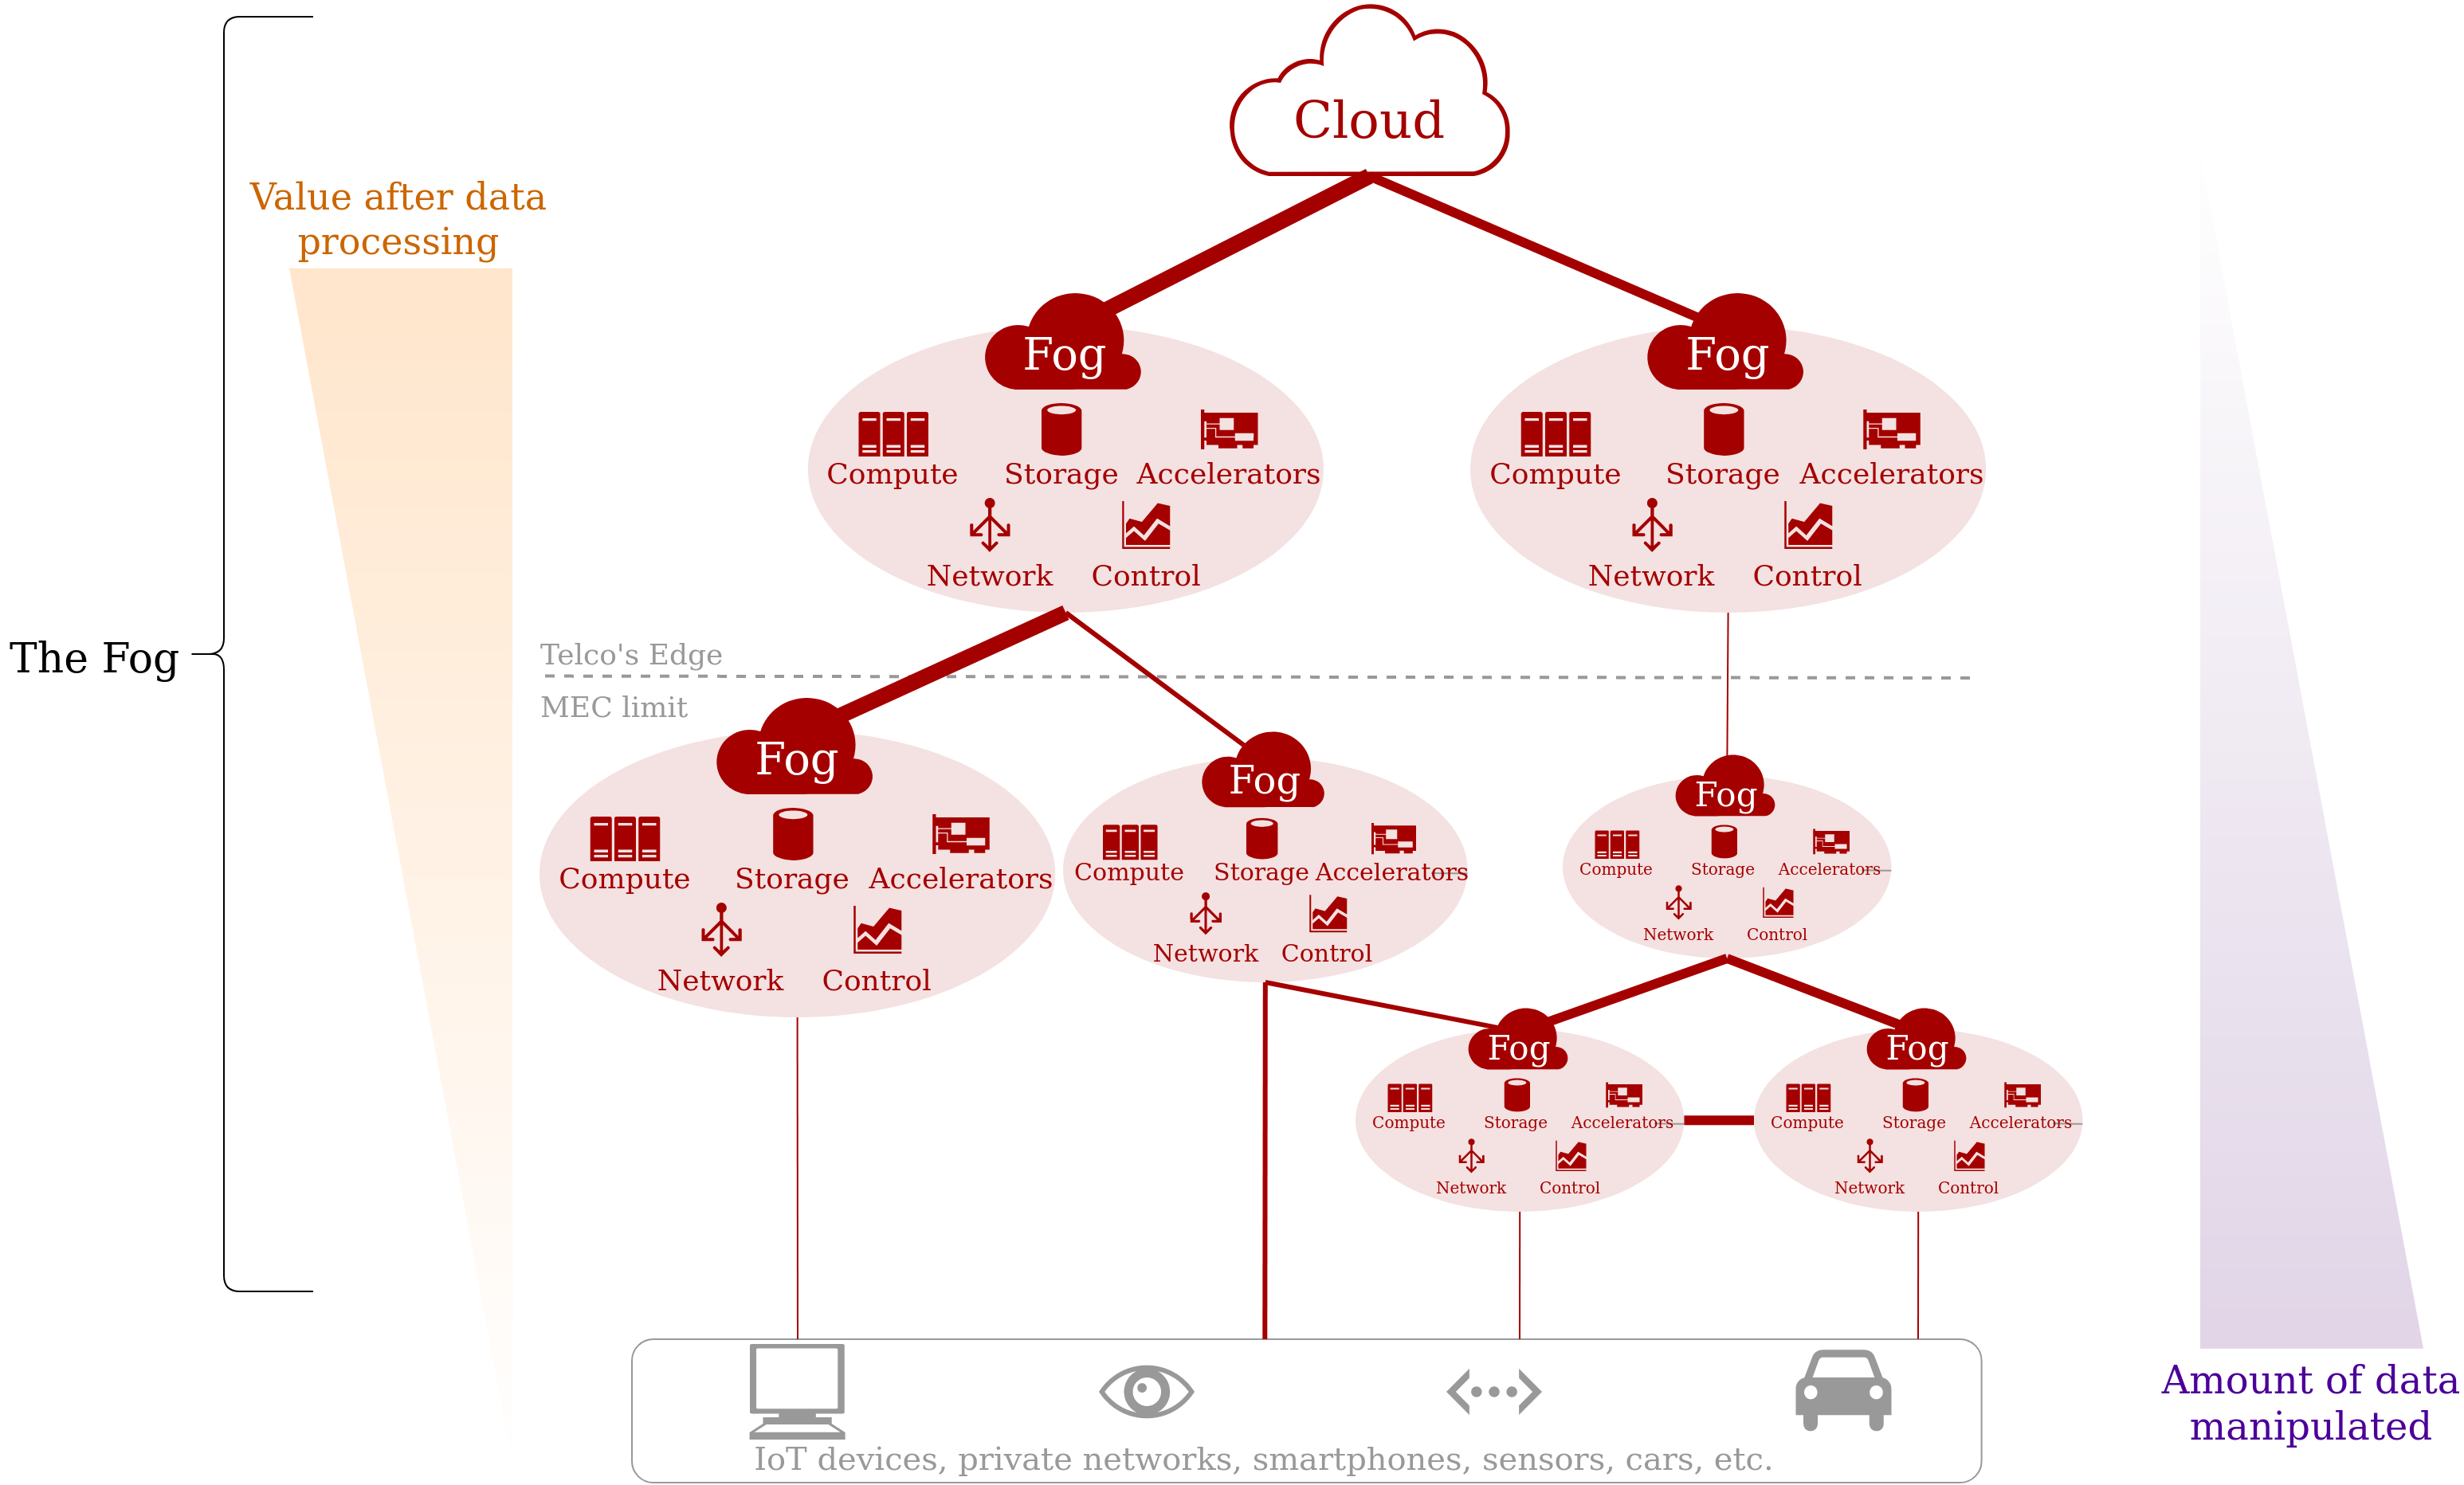
\includegraphics[width=0.78\textwidth]{./assets/FogArchitecture.drawio.png}
		\caption{A typical hierarchical, architecture based on Fog computing \cite{ieee_standards_association_ieee_2018}}
		\label{fig:fog_archi}
	\end{figure}
	
	\item[Fog computing] is a horizontally distributed architecture aiming to bring both the data plane and the control plane closer to the end-user—the event producer—by exploiting all the computing-enabled places along the cloud-to-things continuum. In other words, Fog creates an immersive distribution of computing, where task execution occurs geographically near the producer, while keeping centralized-dependent heavy processes treated in the Cloud, where it is best handled, cf. \cref{fig:fog_archi}. Fog is different from the previous two other edge-only approaches as it provides tools for distributing, orchestrating, managing and securing both resources and services across networks and devices living in the continuum, while also thriving there.
	
	Back in \citedate{bonomi_fog_2012}, Cisco introduced the key characteristics of Fog thanks to \citeposs{bonomi_fog_2012} paper:
	\begin{enumerate}[(i)]
		\item low-latency and location awareness;
		\item wide-spread geographical distribution;
		\item mobility;
		\item very large number of nodes;
		\item dominance of wireless access;
		\item real-time and streaming applications as first-class citizens;
		\item heterogeneity of the nodes (single boards computers or coming with hardware acceleration modules such as a \gls{GPU}, etc.).
	\end{enumerate}
	The Fog initiative is now backed by the OpenFog Consortium \cite{ieee_standards_association_ieee_2018} whose members include ARM, Cisco, Dell, Intel, Microsoft and Princeton University \cite{chiang_fog_2016}.
\end{description}

The benefits are similar for all the paradigms \cite{ahmed_fog_2019, ai_edge_2018}:
\begin{enumerate}[(1)]
	\item latency reduction;
	\item bandwidth optimizations;
	\item computational offloading;
	\item privacy and security through on-premise exploitation;
	\item service management as a middleware;
	\item edge-device monitoring;
	\item energy efficiency-enabling vector;
	\item cost savings through platform acquisition;
	\item content caching.
\end{enumerate}

While all these concepts focus on exploiting the edge of the networks to achieve similar goals constrained by similar challenges, only Fog exploits all the continuum and considers Cloud as much as the edge—and further than it. However, only \gls{MEC} possesses a specification as of 2022. The Fog Consortium acknowledges it and recommends to the Fog contributors to avoid duplication of efforts and focus on aspects not optimized by other approaches. In the long term, the consortium hopes liaisons will form to bring the industry to a common ground \cite{ieee_standards_association_ieee_2018}.

\hypersetup{linkcolor=}
\subsection{Serverless and \acrfull{FaaS}}

Relative to the novelty of the Fog concept, the computing paradigm such a technology would follow is not yet decided. \gls{FaaS} is a Cloud-native technology; would its potential hold in the case of Fog? \cref{sec:literature_review} is full of examples going that way.

\gls{FaaS} is a concept that allows the application developer to only focus on the business logic and not provisioning of the resources \cite{redhat_what_2020}. As its name suggest, the base unit is a function—like the one we use everywhere in computing. This is where its resemblance with microservices shines the most, because the application is cut in those base units, usually stateless. However, provisioning, scaling, capacity management is not the developer's burden anymore, and the Cloud provider is happy to inherit it as he can then optimize his architecture, costs, configuration and enable a global management with much finer-grained control than with \gls{PaaS} or \gls{IaaS}.

\gls{FaaS} should not be confounded with \emph{serverless}, which is its parent concept. \gls{FaaS} concentrates on an event-driven computing-focused aspect. Once an event triggers the platform, the function is started. This is where serverless is much more general, because it comprises compute, storage, database, messaging, API gateways, etc. in its scope. The rest is still the same: configuration, management and billing are invisible for the user \cite{ibm_faas_2019}.

In the case of Fog, serverless and \gls{FaaS} mean resource-constrained environments decide how to manage their resources and only have to handle small slices of one's application, thanks to the division in functions \cite{bermbach_auctionwhisk_2021}.

The introduction of serverless and \gls{FaaS} contributes to new challenges, especially mixed with Fog. To name the most meaningful challenges \cite{kjorveziroski_iot_2021}:
\begin{enumerate}
	\item \emph{cold-starts}, the time spent preparing the runtime before executing the function in it;
	\item \emph{scheduling} and handling different frequencies of execution, provisioning and halting;
	\item \emph{deployment}, where to store the functions, their data, their states, etc.;
	\item \emph{performance} and the underlying difficulties caused by languages and virtualization techniques (\gls{VM}, containers, WASM);
	\item \emph{vendor lock-in} and dependency on only one provider;
	\item \emph{security \& isolation} that is especially true under resource constraints \cite{maurice_hello_2017};
	\item \emph{improvement to function chaining / combination} with non-trivial ways to manage performance (latency, etc.) and costs \cite{elgamal_costless_2018};
	\item \emph{support for hardware acceleration (\gls{GPU}, \gls{AI})}.
\end{enumerate}

\subsection {Applications}

\begin{table}[t]
	\fontsize{10}{8}\selectfont
	\begin{tabular}{@{} p{3cm}|p{12cm} @{}}
		Economic sector & Description
		\\[2ex]
		\cmidrule[1pt]{1-2}
		%		Transportation 
		%		& LiveMap provides fine-grained details about road conditions thanks to vehicular updates \cite{hu_live_2017}.
		%		\\
		%		Health 
		%		& Stroke detection thanks to Fog-distributed fall-detection algorithms, stroke mitigation and splits task detection between smartphones and Cloud servers \cite{hu_survey_2017}.
		%		\\
		Caching
		& Video streaming file caching in edge networks \cite{ma_understanding_2017}.
		\\
		Augmented Reality
		& Track and display the positions of physical objects not in the physical field of view of a user in the context of smart cities. The objects are displayed on smart glasses. Real-time processing is possible thanks to edge nodes processing neighboring camera feeds \cite{rausch_towards_2021, rausch_cognitivexr_2020}.
		\\
		Entertainment
		& Avoid the requirements of installing games on the computers and utilize Fog nodes with hardware acceleration to render video-games \cite{lin_cloudfog_2017}.
		\\
		Smart cities
		& Integration of Fog nodes in smart buildings that would provide the exploitation architecture for new use cases towards better energy efficiency, lower operational costs, etc. thanks to the processing of existing sensors in buildings \cite{ieee_standards_association_ieee_2018}.
		\\
		%		Supply chains 
		%		& Create the ability for delivery drones to collaborate and make operational changes and adjustments in response to anomalies \cite{openfog_consortium_out_2018}.
		%		\\
		%		Smart factories 
		%		& Make smarter brewing thanks to intelligent nodes able to scale and replicate key functions to a production process with large fluctuations in demand periods \cite{openfog_consortium_process_2018}.
		%		\\
		Energy, civil, environment industries
		& Enable real-time subsurface monitoring to better understand subterranean dynamics that would pose threat or be opportunities for oil, gas and geothermal exploitation and exploration \cite{openfog_consortium_real-time_2018}.
		\\
		%		Smart grid 
		%		& Allow the processing of home-based \gls{IoT} closer to the home in question rather than processing the data in another country's Cloud datacenter \cite{chen_design_2018}.
		%		\\
		%		Agriculture 
		%		& Enable a high-precision smart irrigation system for agriculture thanks to optimizations of the irrigation system computed all along the Edge-to-Cloud continuum \cite{noauthor_swamp_nodate}.
		%		\\
		%		Security (IT, physical) 
		%		& Enable a hardware accelerated antivirus to be executed remotely on a close Fog node rather than on the constrained smartphone where it would normally not be able to \cite{deyannis_enabling_2018}.
		%		\\
		\cmidrule[1pt]{1-2}
	\end{tabular}
	\caption{Insight about Fog applications \cite{ahmed_fog_2019}}
	\label{tab:applications}
\end{table}

Fog is envisioned as a way to avoid sending massive amounts data far away and is predicted to be efficient into bringing low-latency and even real-time applications to life \cite{ahmed_fog_2019}. However, no general Fog platform is yet publicly known. \citet{ahmed_fog_2019} have presented an in-depth review of applications. Some of their examples are described in \cref{tab:applications}.

\citet{ahmed_fog_2019} also identify Fog deployment models, similar to the Cloud landscape. Those models can be classified into:
\begin{enumerate}[(a)]
	\item \emph{private Fog} where execution exclusivity is for one user, as well as the hardware's responsibility;
	\item \emph{public Fog}, the opposite, usable by the grand public;
	\item \emph{community Fog}, exclusive to the member of a community;
	\item \emph{hybrid Fog}, which is a mix of all the previous and usually serves scaling purposes.
\end{enumerate}
This variety of models caused by accessibility-related constraints on physical Fog nodes indicates a need for cooperation of the nodes, i.e., bring the ability to connect private nodes with public/community ones using a standard set of protocols and market methods to trade computing power and resources in real-time. Some propositions even consider the creation of an edge network not relying on \glspl{ISP} \cite{bermbach_towards_2021}.

\section{Platforms}
\label{sec:platforms}

A variety of platforms exist to accommodate Fog with the current state of industrial applications. Most of them are focused on a private usage. The node is owned by only one user that exploits a small park of nodes for her only benefit. However, many options—especially the \gls{OSS}—ones can offer the feature of modification and extension needed to bring the Fog paradigm to the next step in an open/reproducible research way. For now, most of these platforms are derivatives of successful Cloud-based ones. This state-of-the-art leads to the technical challenges of running this kind of platform in a resource-constrained environment at the edge.

\subsection{Commercial focus}

These proprietary platforms are published by Cloud giants. The list includes, but is not limited to: Amazon AWS Greengrass \cite{noauthor_aws_nodate}, Microsoft Azure IoT Edge \cite{noauthor_iot_nodate} and Google IoT Core \cite{noauthor_cloud_nodate}. Usually these platforms connect to their provider's cloud as another premium service. The use is then exclusive to the developer connecting these platforms to her subscribed plan. The functionalities offered can be close to \gls{FaaS} in the Cloud, but triggered and processed closer to the data source \cite{elgamal_costless_2018}.

\hypersetup{linkcolor=}
\subsection{\acrfull{OSS}}
\gls{OSS} projects offer more transparent platforms. This is the case of Apache OpenWhisk \cite{noauthor_apache_nodate}. It has been started by IBM and then made publicly available through an Apache 2.0 license. This kind of platform is preferred in the era of open-research for obvious reasons as well as limiting an existing Cloud problem: vendor lock-in \cite{kjorveziroski_iot_2021}. Adaptations have been made to retain the benefit of the source code while running on the more resource-constrained Fog nodes. The project is named Lean OpenWhisk \cite{breitgand_lean_2018}.

Another axis of development focuses on a variety of Kubernetes extensions \cite{bocci_secure_2021}, to name a few: Fission, Kubeless, Knative, OpenFaaS, Nuclio.

Other works have focused on the opposite problem. Instead of adapting the Cloud paradigm to the Edge, Edge-native platforms have started to appear. \citet{pfandzelter_tinyfaas_2020} shows better performances than Lean OpenWhisk. While the work is significant, could it ever reach the industrial maturity level of platforms such as OpenWhisk or Kubernetes once their complete adaption will be achieved? \citeposs{george_nanolambda_2020} NanoLambda is another example of a small platform placed at the Edge. Though not compared, it would extend the reach of Fog to Clusters of IoT devices by making \glspl{SoC} such as Espressif's ESP8266 \cite{noauthor_esp8266_nodate} able to host \gls{FaaS} platforms, thus enabling a closer layer of processing right inside \gls{IoT} networks.

\section{Function placement}
\label{sec:placement}

\subsection{Literature review \label{sec:literature_review}}

This section is dedicated to the literature contributing to strategies for the placement of functions (or similar objects) in the Fog and relevant environments. Placement-related decisions take place in platforms executed on nodes, thus the selection of papers is focused on exploitable strategies found in platforms. A number of contributions has been extracted from \citeposs{bocci_secure_2021} survey.

\begin{description}[leftmargin=10pt]
	\item[\citet{cheng_fog_2019}] defines \textit{Fog functions} as a new \gls{FaaS} platform. The authors note data locality is important. Data are observed to be linked with variable
	\begin{enumerate}[(i)]
		\item entity size;
		\item entity refresh rate;
		\item task complexity;
		\item task running-time;
		\item task priority;
		\item task novelty.
	\end{enumerate}
	The authors also identify what a data-intensive Fog framework should provide:
	\begin{enumerate}[(a)]
		\item data discovery and routing fine-grained to the content of the data;
		\item function triggering solely based on the availability of the input data;
		\item dynamic placement of either data or code to the best processing place;
		\item data dependency as the function composition driver.
	\end{enumerate}
	Nodes are Edge-based or cloud-based. Discovery and orchestration is centralized onto a particular node. The orchestrator is aware of data flowing to its members. It then decides where to execute each function. Data is then routed to that node and processing takes place.
	
	\item[\citeposs{baresi_paps_2019}] \gls{FaaS} platform is focused on low-latency, data-intensive use cases. \cite{baresi_towards_2019} identify multiple challenges to the creation of a \gls{MEC} platform by the research community, it comprises
	\begin{enumerate}[(i)]
		\item resource management;
		\item placement \& migration of application components and services between platforms;
		\item scheduling of computation and offloading from mobile and \gls{IoT} devices.
	\end{enumerate}
	The paper defines a \gls{SEP} that answers a list of requirements:
	\begin{enumerate}[(a)]
		\item low-latency computation offloading;
		\item inter-platform collaboration to ensure \gls{SLA} deadlines;
		\item latency optimization to enable real-time communications;
		\item opportunistic data analysis for anticipation;
		\item edge coordination to enforce location awareness;
		\item stateful partitions to extend \gls{FaaS} support.
	\end{enumerate}
	The authors then proceed to create a prototype implementing each of those points. Their solution is deployed on OpenWhisk. They observe a need to reduce latency, especially in real-time scenarios.
	
	\citet{baresi_paps_2019, baresi_paps_2021} extend this work with the \gls{PAPS} platform while advocating for a decentralized approach to increase speed of control.
	The architecture is divided into three layers:
	\begin{enumerate}[(1)]
		\item A supervisor node that knows the global topology. Its responsibility is to form communities of nodes;
		\item A community is an aggregation of nodes having a latency under a defined threshold. It is in charge of making sure \glspl{SLO} are reached and \glspl{SLA} not violated. The functions processed by the community are allocated by a leader. This centralized approach avoids the need of a more complex protocol while using well known optimal centralized techniques;
		\item Local nodes then receive the responsibility of their allocated resources back, along with the function execution and its \gls{SLO} that the platform must not break, while also not breaking other applications'.
	\end{enumerate}
	So each node actually micromanages its allocated functions and their fluctuations the best they can, while still respecting the leader's decision and global point of view.
	
	Following the theory, and after a promising simulation, \citet{baresi_paps_2021} implements \gls{PAPS} on top of Kubernetes and OpenFaaS. Their conclusion is their partitioning allows for guarantees that decentralized heuristics cannot provide, while still doable in practice, unlike a fully centralized architecture. They also point out they can handle highly fluctuating workloads while acknowledging reactivity of nodes is a challenge due to their use of containers.
	
	\item[\citet{cicconetti_decentralized_2021}] propose a decentralized platform to minimize response times while respecting short- and long-term fairness in stateless task assignations. Their platform does not extend to the Cloud and integrates by the standards of the \gls{MEC} model. An edge device is connected to an edge router that submits the stateless task request to an edge computer. The router decides autonomously where to forward the task in his known pool of compute-enabled nodes. The router proceeds to two actions. It updates the weights by measuring a rolling average of routed function response times submitted to computing nodes. Then it chooses a destination, avoiding congested paths thanks to data provided by a \gls{SDN} controller supervising the network. Three different algorithms have been evaluated to route tasks, namely:
	\begin{enumerate}[(i)]
		\item \label{cicconetti_li} \gls{LI}—always selects the minimum cost node;
		\item \label{cicconetti_rp} \gls{RP}—selects a random node with a probability proportional to the weighted path to that node;
		\item \label{cicconetti_rr} \gls{RR} combines the proportional benefits of \cref{cicconetti_rp} with the greediness of \cref{cicconetti_li}.
	\end{enumerate}
	\cref{cicconetti_rr} achieves both short- and long-term fairness, while \cref{cicconetti_rp} only the latter. \cref{cicconetti_li} is the worst performer.
	The authors conclude \gls{SDN} plays a capital role in the system. Under load variations, performance is equally good as in regular distributed systems. Finally, exploration of hierarchical task forwarding in a simulated test-bed with OpenWhisk offers interesting scalability perspectives.
	
	\item[\citeposs{tasiopoulos_fogspot_2019}] FogSpot allows the provisioning of heavily stateful \glspl{LLA}—\glspl{VM} that can neither be migrated nor suspended—on Fog nodes along the path of an Edge device's request to its default execution location: the Cloud. That way either the request is accepted and provisioned or it is forwarded to a further node. If it only gets forwarded, it ends up executed in the Cloud.
	Each node hosts a trusted market. A \gls{LLA} request is a truthful bid that shows its willingness to pay per unit of time and its value in the \gls{QoS} gain that would be observed if the request was to be accepted and the application served on this particular node. Of course, the further the request is from the edge, the lower the bid as the utility decreases, until it finally reaches 0 and the Cloud.
	Each node can either choose to maximize its revenue or its social welfare. Those strategies are reflected in the used Dutch auctions termination's conditions. Such auctions are employed to keep processing requests on the spot, without having to queue and to wait anywhere along the request's path. A depth analysis of executions is conducted by the authors and reveals that the first strategy leads to more gain for the node's provider but with uncertainties on the prices when executed in a decentralized/uncoordinated way while the second one will try to fully exploit the capacity of the node and provide a stable solution in an uncoordinated space.
	
	\item[\citeposs{mutichiro_qos-based_2021}] contribution is STaSA, a scheduler developed for KubeEdge to be executed in a \gls{MEC} community of nodes: multiple nodes aggregated around a leader because of their proximity latency-wise, here thought to be in a server rack. The scheduler is introduced as a way to respect as much as possible applications' \gls{QoS} requirements. Other objectives are also considered: node utilization maximization, cost minimization (compared to standard Cloud) and service-time optimizations. This problem is NP-hard. STaSa is built upon the \gls{ACO} probabilistic model to place containers—called functions throughout the article. The model has been tweaked, especially during the pheromone updates and calculations. In principle, ants are dispatched to the nodes to find the best suitable placement. On their way back they leave a pheromone trace. Its intensity/weight depends on a number of factors the ant found in the node (CPU/RAM utilization, latency, \gls{QoS}, etc.). Termination is reached when either a threshold is reached or when the best placement is found: when the minimal cost is thought to have been found. Practical implementations showcase better results than baseline \gls{ACO} and First Come First Served strategies.
	
	\item[\citet{palade_swarm-based_2020}] theorized the idea of using the \gls{ACO} meta-heuristic algorithm for function placement in \gls{MEC}. The content can be directly compared to \cite{mutichiro_qos-based_2021}, noting that the first dates back to \citedate{mutichiro_qos-based_2021} whereas the latter is older by a year (\citedate{palade_swarm-based_2020}). However, \cite{palade_swarm-based_2020} concentrates explicitly on \gls{MEC}. They also succeed to show this approach leads to less overall latency. They argue this gain largely mitigates the failure to find an optimal load-balancing and a “sub-second” higher execution time.
	
	\item[\citet{rausch_optimized_2021}] introduce Skippy. This function scheduler is based on annotations present in the functions code, such as an indication of hardware specific dependencies. It assumes a lesser level of control about the cluster status and functions requirements as it is observed in practice in the industry. The authors present their work as an improvement over the default greedy multi-criteria decision-making Kubernetes online scheduler \footnote{An online scheduler has no knowledge of future arrivals.} algorithm. They add four new aspects—functions:
	\begin{enumerate}[(i)]
		\item \emph{LatencyAwareImageLocalityPriority} that favors nodes where access to the container registry is quick enough;
		\item \emph{DataLocalityPriority} that influences the location of the function based on the predicted data transfer;
		\item \emph{CapabilityPriority} that is aware of hardware accelerations requirements for functions;
		\item \emph{LocalityTypePriority} that favors Cloud or Edge placement if required by the user.
	\end{enumerate}
	
	In a second part of their paper, the authors implement a simulator to optimize the weights of their scheduler at scale. Their implementation allows for a single code basis as the simulator calls the Skippy scheduler directly.
	
	Simulations are executed over different plausible scenarios generated by a topology synthesizer as no large-enough test-bed exists.
	
	Conclusion is that their work enables locality-sensitive function placement resulting in a better utilization of the network bandwidth, even when a trade-off of execution cost for application latency have been observed. The authors also conclude that improving placement quality counterbalances the loss in scheduler performance to do it.
	
	%TODO maybe merge the two references, cf https://onlinelibrary.wiley.com/doi/full/10.1002/spe.3058 which is the newer version of the paper, so ...
	\item[\citet{bermbach_towards_2021}] are interested in the issue of function placement in multiple geo-distributed sites in Fog fashion. From their perspective, a serverless—particularly a \gls{FaaS} approach—is relevant because provisioning is done in small slices instead of full containers or \glspl{VM}. Additionally, moving functions back and forth between Cloud and the Edge is easier due to their stateless natures. Their framework will use an auction-based approach, as they argue this kind of approach showed success in the past.
	Bidding is done when developing the function. Two bids are attached
	\begin{enumerate}[(a)]
		\item \emph{Data storage bid}, i.e., the price the developer is willing to pay for a node to store his executable per unit of time;
		\item \emph{Processing bid}, ie the price the developer is willing to pay per for a node to execute his function.
	\end{enumerate}
	These bids are able to translate a preference for Cloud, Edge or an indicated node. Accepted bids are then paid over a minimum price, as a surcharge. A second-price auction is deemed to be the better option here.
	
	The authors then proceed to prove this approach works by developing a simulator and conclude auction-based function assignation and storage are an efficient mechanism in Fog-enabled contexts where there is both a lack of processing and storage capacity.
	
	In a following journal paper, \citet{bermbach_auctionwhisk_2021} identify four constraints to implement this model:
	\begin{enumerate}[(i)]
		\item auctions process in batches, there is a need of a window of time when the system estimates refusing functions is required;
		\item storage space calculations do not depend on the number of functions but on their sizes, especially as their metadata is expected to grow after each execution;
		\item estimating the number of supported concurrent function executions as some functions will be either under or over-provisioned;
		\item a node is required to know its neighbors, especially the one leading the path towards the Cloud; however, this needs to be achieved despite node failures and parameter changing over time.
	\end{enumerate}
	
	Then the authors present a prototype named \emph{AuctionWhisk}, based on OpenWhisk (also supporting the \emph{Lean} flavor). They experiment on a limited setup consisting of an edge, an intermediary and a cloud node.
	
\end{description}

Other platforms present active management of a node's function execution, e.g., reclaim resources or grant more, this is the case of \gls{LaSS} developed by \citet{wang_lass_2021}. More classical approaches are also taken, as \citeposs{elgamal_droplet_2018} DROPLET that uses an underlying centralized graph optimization algorithm to place functions.

\section{Curated list of unresolved problems}
\label{sec:curated}

%\newcommand{\tabred}{-4pt}
%\newcommand*\rot{\rotatebox[x=2cm]{90}}
\newcommand*\rot{\rotatebox{90}}
\newcommand*\OK{\ding{51}}
\begin{table}[t] \centering
	\fontsize{10}{8}\selectfont
	\begin{tabular}{@{} cl*{3}c|*{3}c|*{9}c @{}}
		&                                                                                             & \multicolumn{3}{c}{Architecture} & \multicolumn{3}{c}{Method} & \multicolumn{8}{c}{Scheduling features}                                                                                                                                                                                                                                                                                                                                                                                                                                                                         \\[2ex]
		&                                                                                             & \rot{Decentralized}              & \rot{SLA/SLO support}      & \rot{Fog (vs \gls{MEC})}                & \rot{Auction} & \rot{(Meta-)heuristic} & \rot{\shortstack[l]{Multi-landlord \cr compatibility}} & \rot{Geo-aware} & \rot{Execution latency} & \rot{\shortstack[l]{Service-costs \cr (RAM, CPU, etc.)}} & \rot{\shortstack[l]{Network awareness \cr(topology, congestion-aware, etc.)}} & \rot{Data source aware strategy} & \rot{\shortstack[l]{Heterogeneous hardware \cr (GPU, etc.)}} & \rot{Image registry awareness} & \rot{Stateful} & \rot{Security awareness} \\
		\cmidrule{2-17}
		& Cheng \textit{et al.}\cite{cheng_fog_2019}                                                  &                                  & \OK                        & \OK                                     &               &                        &                                                        & \OK             & \OK                     & \OK                                                      &                                                                               & \OK                              &                                                              &                                &                &                          \\
		& Baresi \textit{et al.} \cite{baresi_paps_2019, baresi_towards_2019, baresi_paps_2021}       &                                  & \OK                        &                                         &               &                        &                                                        &                 & \OK                     & \OK                                                      & \OK                                                                           &                                  &                                                              &                                &                &                          \\
		& Cicconetti \textit{et al.} \cite{cicconetti_decentralized_2021}                             & \OK                              &                            &                                         &               & \OK                    & \OK                                                    &                 & \OK                     &                                                          & \OK                                                                           &                                  &                                                              &                                &                &                          \\
		& Wang \textit{et al.} \cite{wang_lass_2021}                                                  &                                  & \OK                        &                                         &               &                        &                                                        &                 & \OK                     &                                                          &                                                                               &                                  &                                                              &                                &                &                          \\
		& Tasiopoulos \textit{et al.}\cite{tasiopoulos_fogspot_2019}                                  & \OK                              &                            & \OK                                     & \OK           &                        & \OK                                                    &                 & \OK                     &                                                          & \OK                                                                           &                                  &                                                              &                                & \OK            &                          \\
		& Mutichiro \textit{et al.} \cite{mutichiro_qos-based_2021} \& \cite{palade_swarm-based_2020} &                                  &                            &                                         &               & \OK                    &                                                        &                 & \OK                     & \OK                                                      &                                                                               &                                  &                                                              &                                &                &                          \\
		\rot{\rlap{~Contributions}}
		& Rausch \textit{et al.} \cite{rausch_optimized_2021}                                         &                                  &                            &                                         &               & \OK                    &                                                        &                 &                         & \OK                                                      &                                                                               & \OK                              & \OK                                                          & \OK                            &                &                          \\
		& Bermbach \textit{et al.} \cite{bermbach_auctionwhisk_2021}                                  & \OK                              &                            & \OK                                     & \OK           &                        & \OK                                                    &                 & \OK                     & \OK                                                      &                                                                               &                                  &                                                              & \OK                            &                &                          \\
		& Elgamal \textit{et al.} \cite{elgamal_droplet_2018}                                         &                                  &                            & \OK                                     &               &                        &                                                        &                 & \OK                     & \OK                                                      &                                                                               &                                  &                                                              & \OK                            &                &                          \\
		\cmidrule[1pt]{2-17}
	\end{tabular}
	\caption{Prominent comparison points between placement frameworks mentioned in \cref{sec:literature_review}}
	\label{tab:placement}
\end{table}
We compare the approaches detailed in \cref{sec:literature_review} on the following three dimensions:
\begin{enumerate}[(1)]
	\item architecture: whether the platform is in favor of decentralizing decision-making, supports \glspl{SLA} or is specifically designed for the Fog;
	\item placement method: what type of strategy is the platform following (heuristic or meta-heuristic based vs centralized algorithms)? Is it an auction mechanism? Is it usable with multiple Fog providers?;
	\item scheduling features: all the considered parameters in the decision-making processes and the studied strategies.
\end{enumerate}
The result is \cref{tab:placement}, from which we can highlight limitations of existing work:

\begin{description}[leftmargin=10pt]
	\item[Lack of \acrfullpl{SLA}] that would cover all the challenges posed by the evolution from Cloud to Fog \cite{chiang_fog_2016, bonomi_fog_2012} and the ones depicted in \cref{tab:placement}:
	\begin{enumerate}[(1)]
		\item \label{item:latency} low / deterministic latency, both at execution and preparation (data transfers for the inputs, outputs, and function themselves);
		\item \label{item:geo} geographical location;
		\item \label{item:network} network bandwidth;
		\item \label{item:uptime} service / network uptime, topology, congestion;
		\item \label{item:heterogeneity} heterogeneity (hardware acceleration, edge preference, etc.);
		\item \label{item:streaming} streaming capacity;
		\item \label{item:costs} service costs (CPU usage, RAM usage, monetary (platform's uptime, usage, level of cooperation with other Fog landlords), etc.);
		\item \label{item:wireless} wireless infrastructure;
		\item \label{item:security} security.
	\end{enumerate}
	\Cref{item:latency} is fairly well represented as seen in \cref{tab:placement}. Looking at the same table, \cref{item:geo,item:network,item:uptime,item:heterogeneity,item:streaming,item:costs} are not well-supported. \Cref{item:security,item:wireless} are not supported to the best of our knowledge, even though the benefits of integration with radio based—broadcasted—transmissions could be interesting. Using \glspl{SLA} and \glspl{SLO} would make application developers know what guarantees they have—or not—on each point as well introducing an economic aspect in the platforms.
	
	\item[Smarter auction-based placement mechanisms] would factorize all the complexity of resource availability, demand, interests and transactions (\glspl{SLA}, \glspl{SLO}) between providers and consumers as well as economics, and embed them in a collaborative dynamic that can be decentralized into multiple marketplaces. \Cref{tab:placement} shows auction mechanisms have been successfully proposed towards such a goal. One should now compare different auction mechanisms to enable real-time transactions guaranteeing fairness, truthfulness and other aspects like giving better access to the user providing the most value to the system of Fog nodes and users (reducing the bandwidth usage, executing a real-time application, etc.). \citet{milgrom_redesigning_2017} proposes depreciating licenses in 5G spectrum division to enable users with high valuations to reserve a channel while letting other users have an uncertainty-prone zero-guarantees usage. The model is dynamic enough for the reserved channel owners to change when their values are superseded by a competitor's, thus driving innovation in the particular case of the radio band usages. Truthfulness is guaranteed because the channel is only rented, meaning the user has to pay the value he gives to the band. Maybe such a model could be introduced in the Fog to allow nodes to have priority functions, that are more valuated, while letting other users the opportunistic, less-costly path.
	
	\item[\gls{FaaS}-specific mechanisms] that would exploit the “cold-start” phenomenon: already provisioned applications can be cached or check-pointed \cite{karhula_checkpointing_2019}.
	Later executions of check-pointed functions at the same node could be accomplished at a lower cost both in time and resources.
	Another rarely-supported feature in \cref{tab:placement} is taking advantage of the physical location of the image registry. Functions can be uploaded either by an end-device, a central Cloud-based registry or a Fog-based, decentralized, one. Another linked problem is about versioning of such distributed/decentralized architectures. How to update functions while avoiding downtimes and conflicts (this problem may get harder when considering that part of the application executes centrally in the Cloud)? One could extend this point to the data source locality awareness, as it is also rare in \cref{tab:placement}.
	
	\item[Security and privacy] as the baseline. Security of both hardware and software is required, to trust the node and the function executing on that node, i.e., making sure an ill-intentioned payload doesn't escape from its enclosure \cite{maurice_hello_2017}. Privacy is another point of interest that is especially relevant when designing auctions, as a node could take advantage of knowing the true valuation it was given by the function. Those two features that should be implemented \emph{by-design} are not currently supported in \cref{tab:placement}.
\end{description}

\iffalse

\section{Plan}

Lack of SLA + Auctions + FaaS specific mechanisms

For an internship -> only 2 firsts could be done in time

Introducing our framework

What do we consider as a context: tree shaped Fog, need for a trusted marketplace

How would one use our framework

Is there any related work particularly work on which we could have been based: Fogflow \cite{smartfog_fogflow_2022} (history ?) + FogBus \cite{deng_fogbus2_2021} as retained candidates (maybe list the others?)

How is this framework working under the hood: fog nodes, marketplace, why rust (language, quality of code, size, performance -> always the Fog in focus + independence from the platform [the code could run on a more embedded device wihtout troubles instead of being limited to Cloud only platform]), the arch using clean architecture, the routing mechanism, the REST \gls{API}, using openAPI + why it is important + open science (have citations for this trend)

How do we run the framework (development using mutlipass, then using grid5000 + Enos \cite{cherrueau_enoslib_2022}) -> what do the script do

What are its benefits

What are its limitations

How do we plan to evaluate it, to validate or not both of the benefits and limitations = two levels for a paper

What are the plans for the future (Thesis + Terra Forma \cite{longuevergne_terra_2022})

\fi

\section{Taking action}
\label{sec:takingaction}

\gls{FaaS}-enabled Fog would allow an applied real world usage of the Fog. However, as depicted in \ref{sec:curated} we identified four main axes of necessary improvements to go this direction:
\begin{enumerate}
	\item introduce \glspl{SLA} that lets the users to set their expectations and have them respected
	\item smarter auction-based placement mechanisms that enable full-scale incentives to both join and compete on the Fog
	\item \gls{FaaS}-specific tools adapted to the Fog
	\item security and privacy
\end{enumerate}.
As this is a research work, we expect “scientific comparison” to be listed

Indeed, the community presents promising placement solutions but fails to both compare them against each other and to test them on real scenarios instead of relying extensively on simulations. Thus it is not clear what to expect from the Fog as of today. This is the first reason why we choose to participate to the community effort producing a framework fit to be experimented upon in preference to being simulated. A second key point is to be able to face implementation issues that would—through simulation—not be observed and remedied.

In the next subsections, we examine our proposed placement mechanism. We will elaborate on the work done on our own open framework. Finally, we will detail how we plan to evaluate this solution and platform against state-of-the-art behaviors.

\subsection{Placing functions in the Fog}

This internship focuses on the execution of a new idea for situating functions in the Fog using economics as the main layer of dialogue between actors, much like what is already in place in the Cloud. After introducing our view of the Fog, we will detail our placement behaviors, how and why we chose to implement our own framework and the evaluation contributions regarding this work.

\subsubsection{Context and challenges}

The Fog is a distributed network made of Fog nodes—computers—that work together to bring latency and bandwidth (among others) benefits to the Cloud customer. In time, the Fog will be so entangled with the Cloud that clients should not be able to discern between executing their applications on the Fog or on the Cloud only. At least when they do not have any explicit requirements making them Fog-reliant. This signifies pricing should as well be indistinguishable from the current offerings and as easy to understand. This also means logistics should be on point: Fog nodes are present everywhere not to degrade the usage made by any applications explicitly depending on them.

This indicates a need to escape the “vendor lock-in” nightmare, where large resource providers are on a single market. But as everyone proposes the same kind of service, each still manages to do it in a proprietary manner, making a multiple-provider scenario hard to reach. This is what we are currently observing in the Cloud, with global companies consuming the Cloud and trying to rely on other providers to avoid downtime, security issues and profit from the best features of both platforms.

Such a problem in Fog would be highly inefficient. It would only signify two things: either all providers are presents at the same location, thus putting a lot of Fog nodes at the same place for no further benefits than pure pecuniary competition. Or it would mean that geographical zones would be exclusive of a handful providers. In each case, it would be a nightmare for the customer to deploy an application at a European-level, for example.

In our work, we consider Fog nodes are owned by different economic actors. This way, both private (enterprises) and public (cities) can provide computational resources to the community, while expecting sufficient gains to be able to sustain this sharing, and to make profits. The more Fog nodes join the network, the more rivalry and the more affordable it is for purchasers to execute applications. We consider that any provider can be in competition, but employing a standard platform to do so, so that it does not hurt the client nor makes the technology useless.

Considering this ownership of fog nodes, as proposed earlier, a good mechanism to introduce contest in a controlled, independent and objective manner are \emph{auctions}. Well-designed auctions can lead to a maximization of social welfare—increase utility for everyone involved—, let participants freely choose their price while making it pointless to lie about the value of the commodities. One last interesting technique is the fairness of the auctions, aka not constantly electing the same winner when multiple have similar bids. In our case, this would not always mean to allocate the same function on the same Fog node when two functions are similar in terms of requirements and bids \cite{kuo_proportionnet_2020}.

\subsubsection{Placing functions}

Placing functions is a challenge. Adding that Fog nodes are independent actors that choose to join the network increases difficulty. Especially since Fog nodes are able to specify their prices and autonomously choose their behaviors. Auctions help to make sure competition is maintained and as such, costs are not artificially set and do not harm the final customer.

Auctions also support translating what metrics are considered important by a Fog node in a single number: the price—that being virtual or real. As an example, Fog nodes near the \gls{IoT} sources—at the edge of the network—could have more concerns about energy usage than fog nodes running off data centers, and so, make high power-consuming clients pay more.

With money in the equation, Fog nodes will not believe each other, as such we need to introduce the first ingredient of our architecture: the \emph{Marketplace}. It is the only software that is trusted by all Fog nodes.

This piece of the framework is the place that will handle the auctioning process and so, the designation of a winner. We do not care about payment at the time, this method being purely for testing purposes\footnote{However, we still anticipate the implementation of such behavior, which is why we introduce this trusted third-party.}.

The Marketplace is the component of the framework which is accessible to the public. It can be thought as a middleware acting as a top gateway to the consumer that wants to deploy and administer their functions.

As the marketplace offers to only oversee functions, clients may need a higher-level solution to coordinate their applications, introducing the “Deployment Manager.” This piece of software would—in the future—be responsible of handling the deployment of the client's application on the Fog. It would be aware of what \gls{IoT} devices are expected as it would know which ones are currently connected to the Fog. Its role would then be to ask the Marketplace to provision functions as it would be deemed necessary from their programming. The idea is to externalize the application managing from the Fog network separates it from the function execution concerns. That way, in case of failure or incapacity to provision part of the application, the task would be handled by a policy specified by the client. This would especially be relevant for the case of a critical application needing to be aware of its ability or inability to be executed. And in such cases transmit the information to a human, for example. Or in a more basic fashion needs to consider changing its requirements to be more adequate to fit the current state of the Fog.

Because we are developing from scratch, we simplified the Fog network topology to be a tree instead of a graph.

\begin{figure}[H]
	\centering
	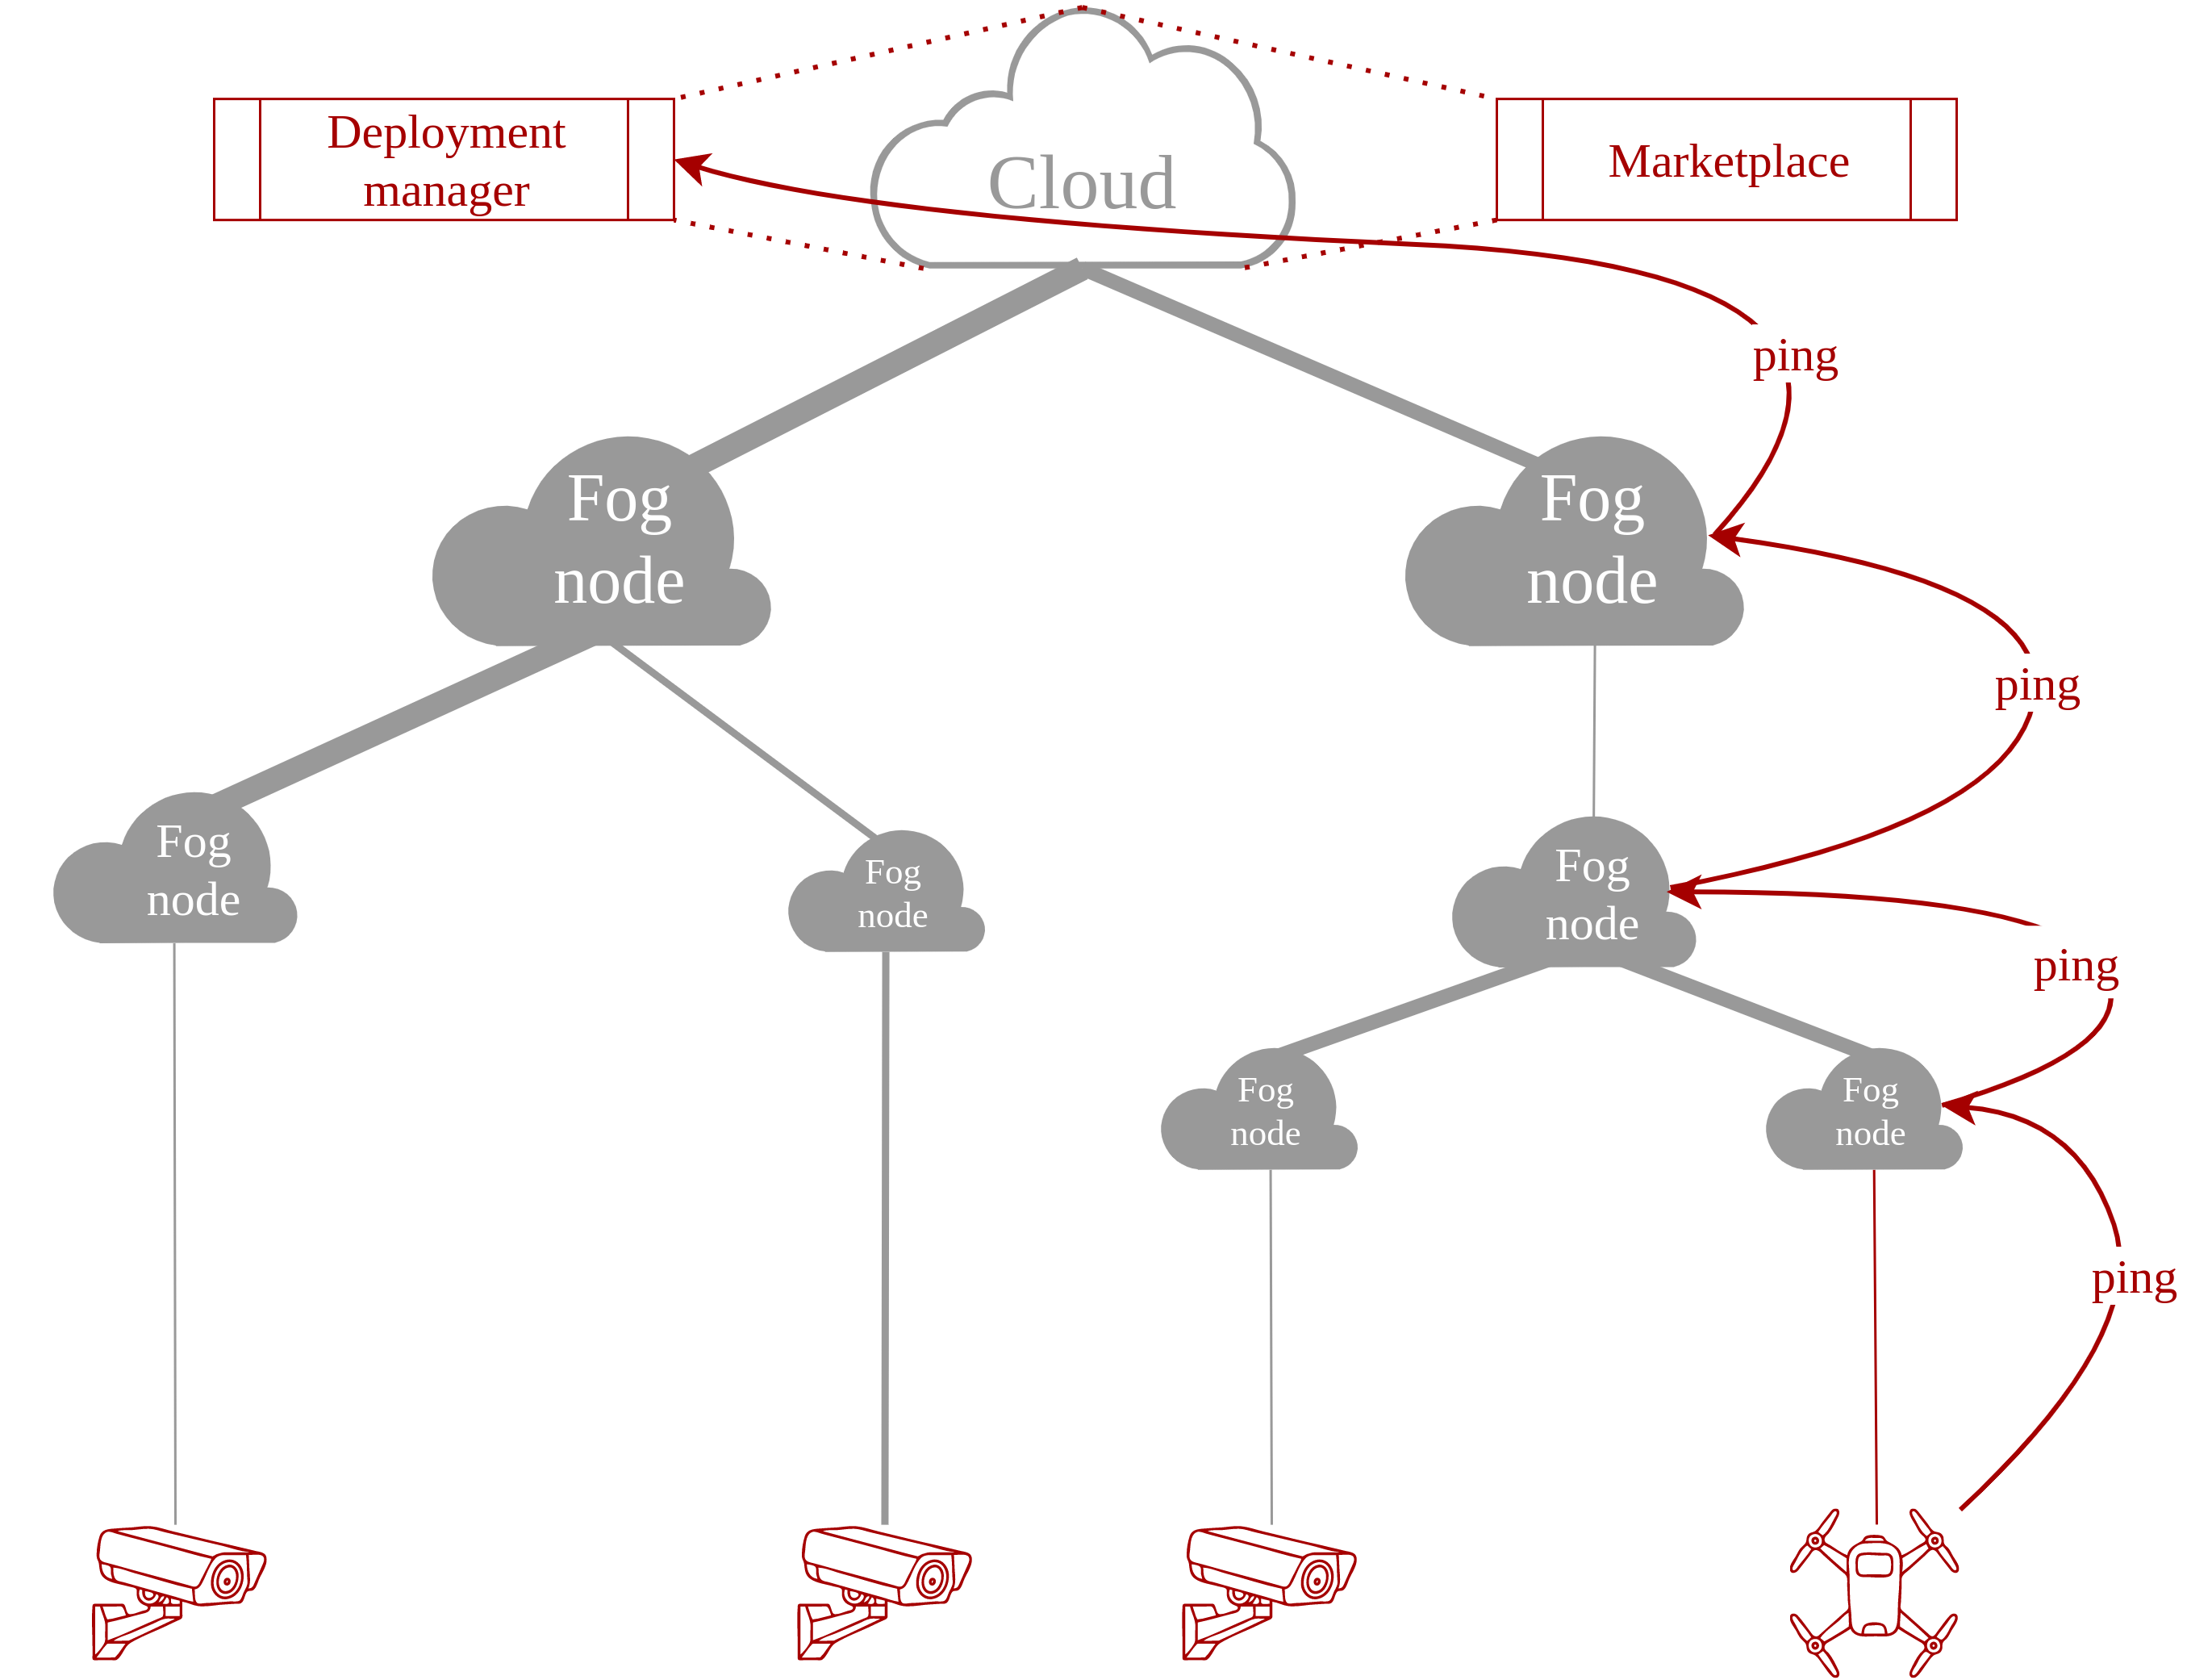
\includegraphics[width=0.65\textwidth]{./assets/OurPlacementOriginal-Page-1.png}
	\caption[Step 0—\gls{IoT} devices just connected]{step 0—\gls{IoT} devices just connected\\
		\textit{Cameras and a drone make the deployment manager aware of their presence by “pinging” it}}
	\label{fig:our_placement0}
\end{figure}
\begin{figure}[H]
	\centering
	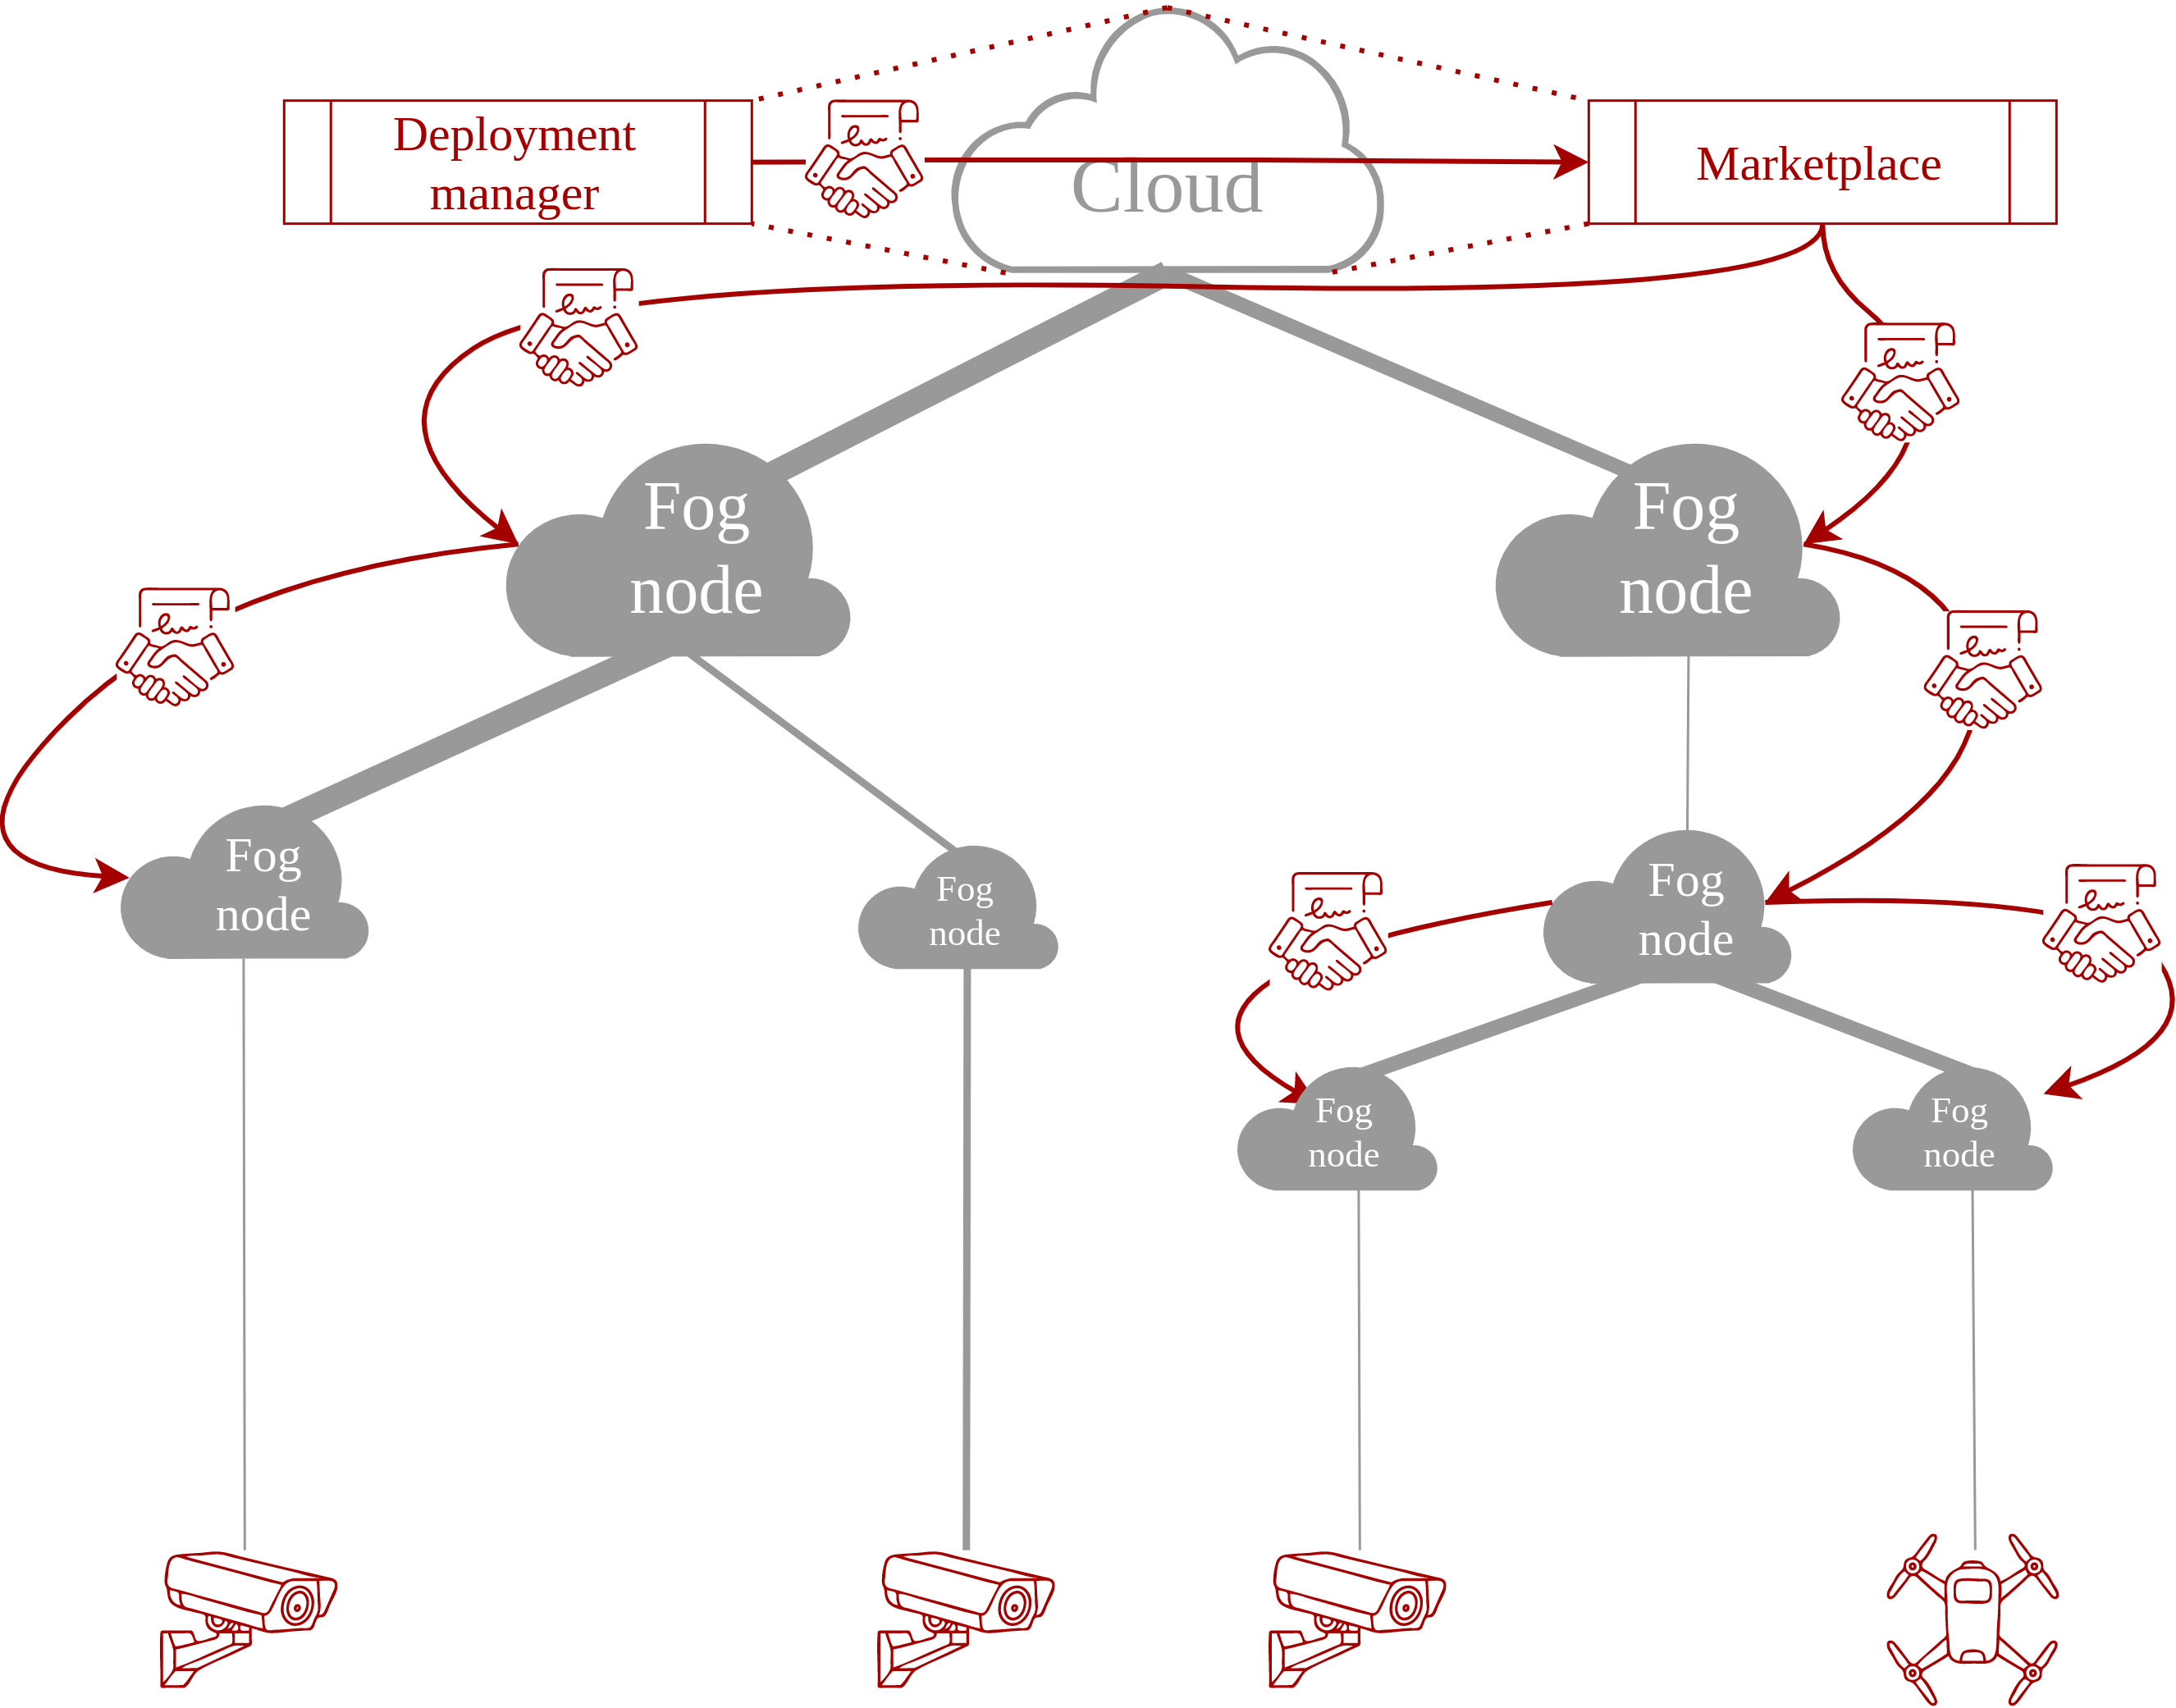
\includegraphics[width=0.65\textwidth]{./assets/OurPlacementOriginal-Page-2.png}
	\caption[Step 1—\gls{SLA} creation and distribution]{step 1—\gls{SLA} creation and distribution\\
		\textit{The Deployment Manager identifies missing functions to be deployed and creates a \gls{SLA} contract describing their requirements (CPU, RAM, latency, etc.). Then sends it to a Fog node that relays to other Fog nodes until a requirement breaks.}}
	\label{fig:our_placement1}
\end{figure}
\begin{figure}[H]
	\centering
	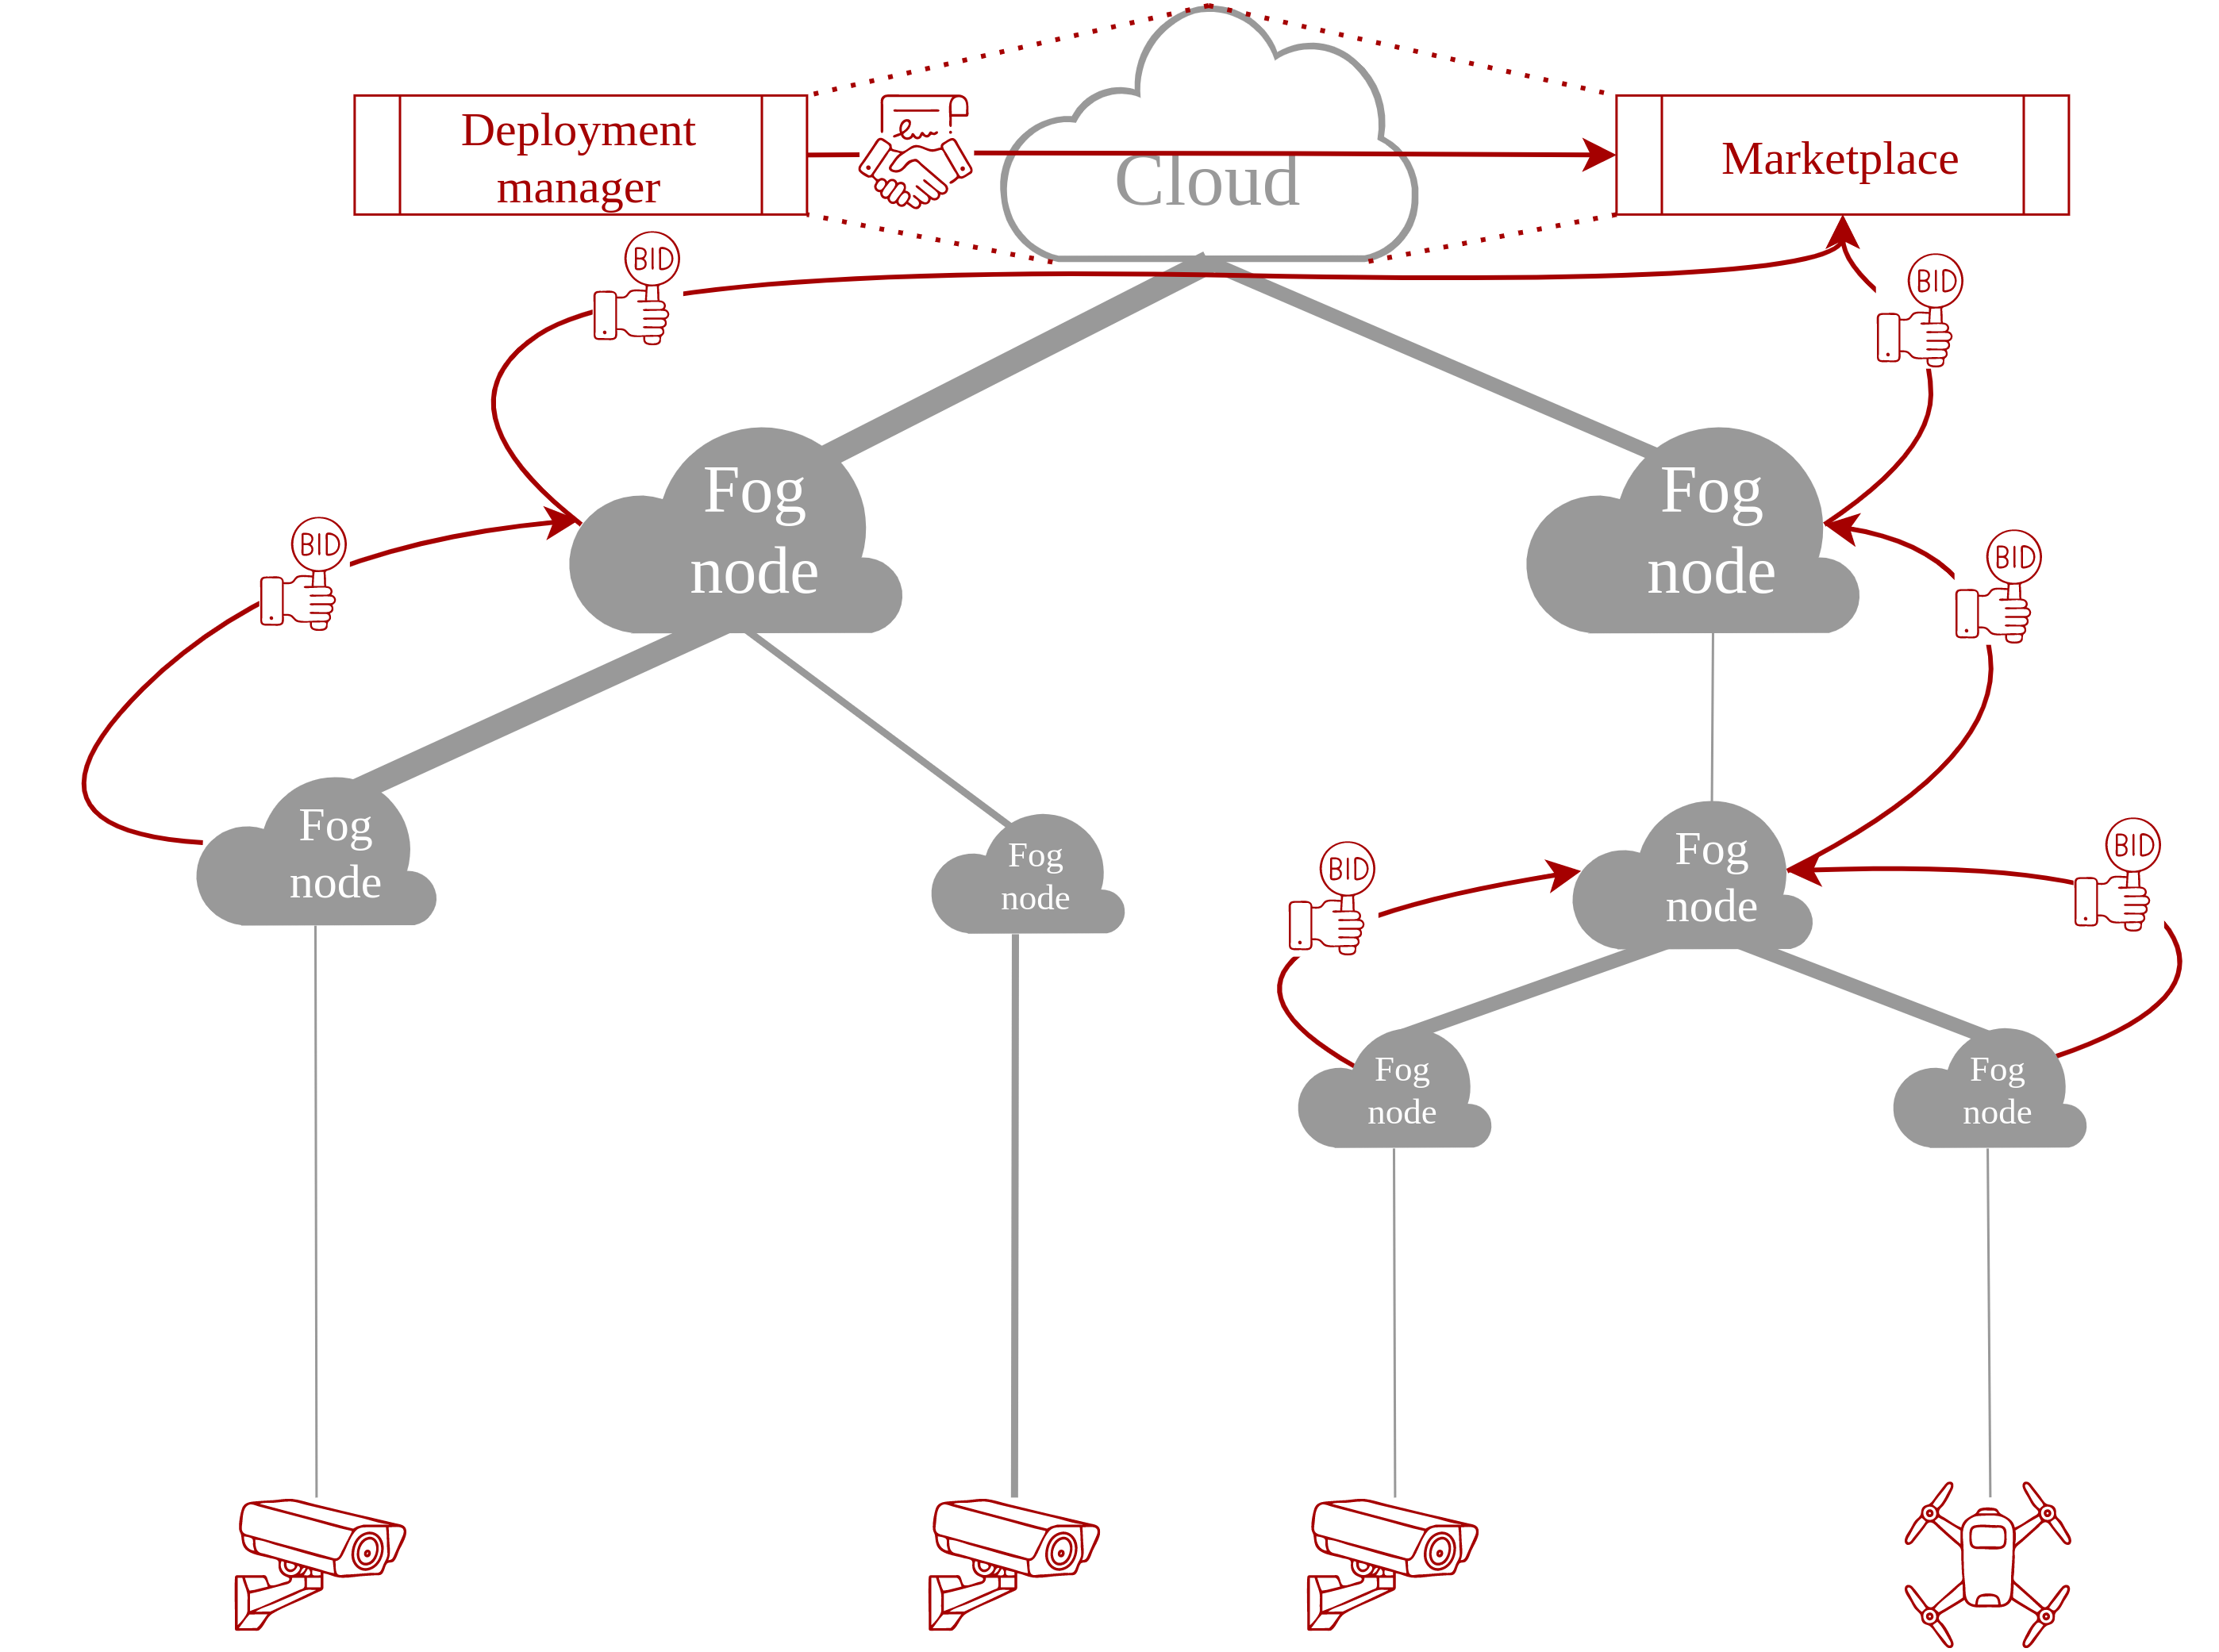
\includegraphics[width=0.65\textwidth]{./assets/OurPlacementOriginal-Page-3.png}
	\caption[step 2—Bidding]{step 2—Bidding\\
		\textit{Upon receiving the \gls{SLA}, each Fog node bid on it and return their price to the marketplace. This represents what they think the function will cost to be executed.}}
	\label{fig:our_placement2}
\end{figure}
\begin{figure}[H]
	\centering
	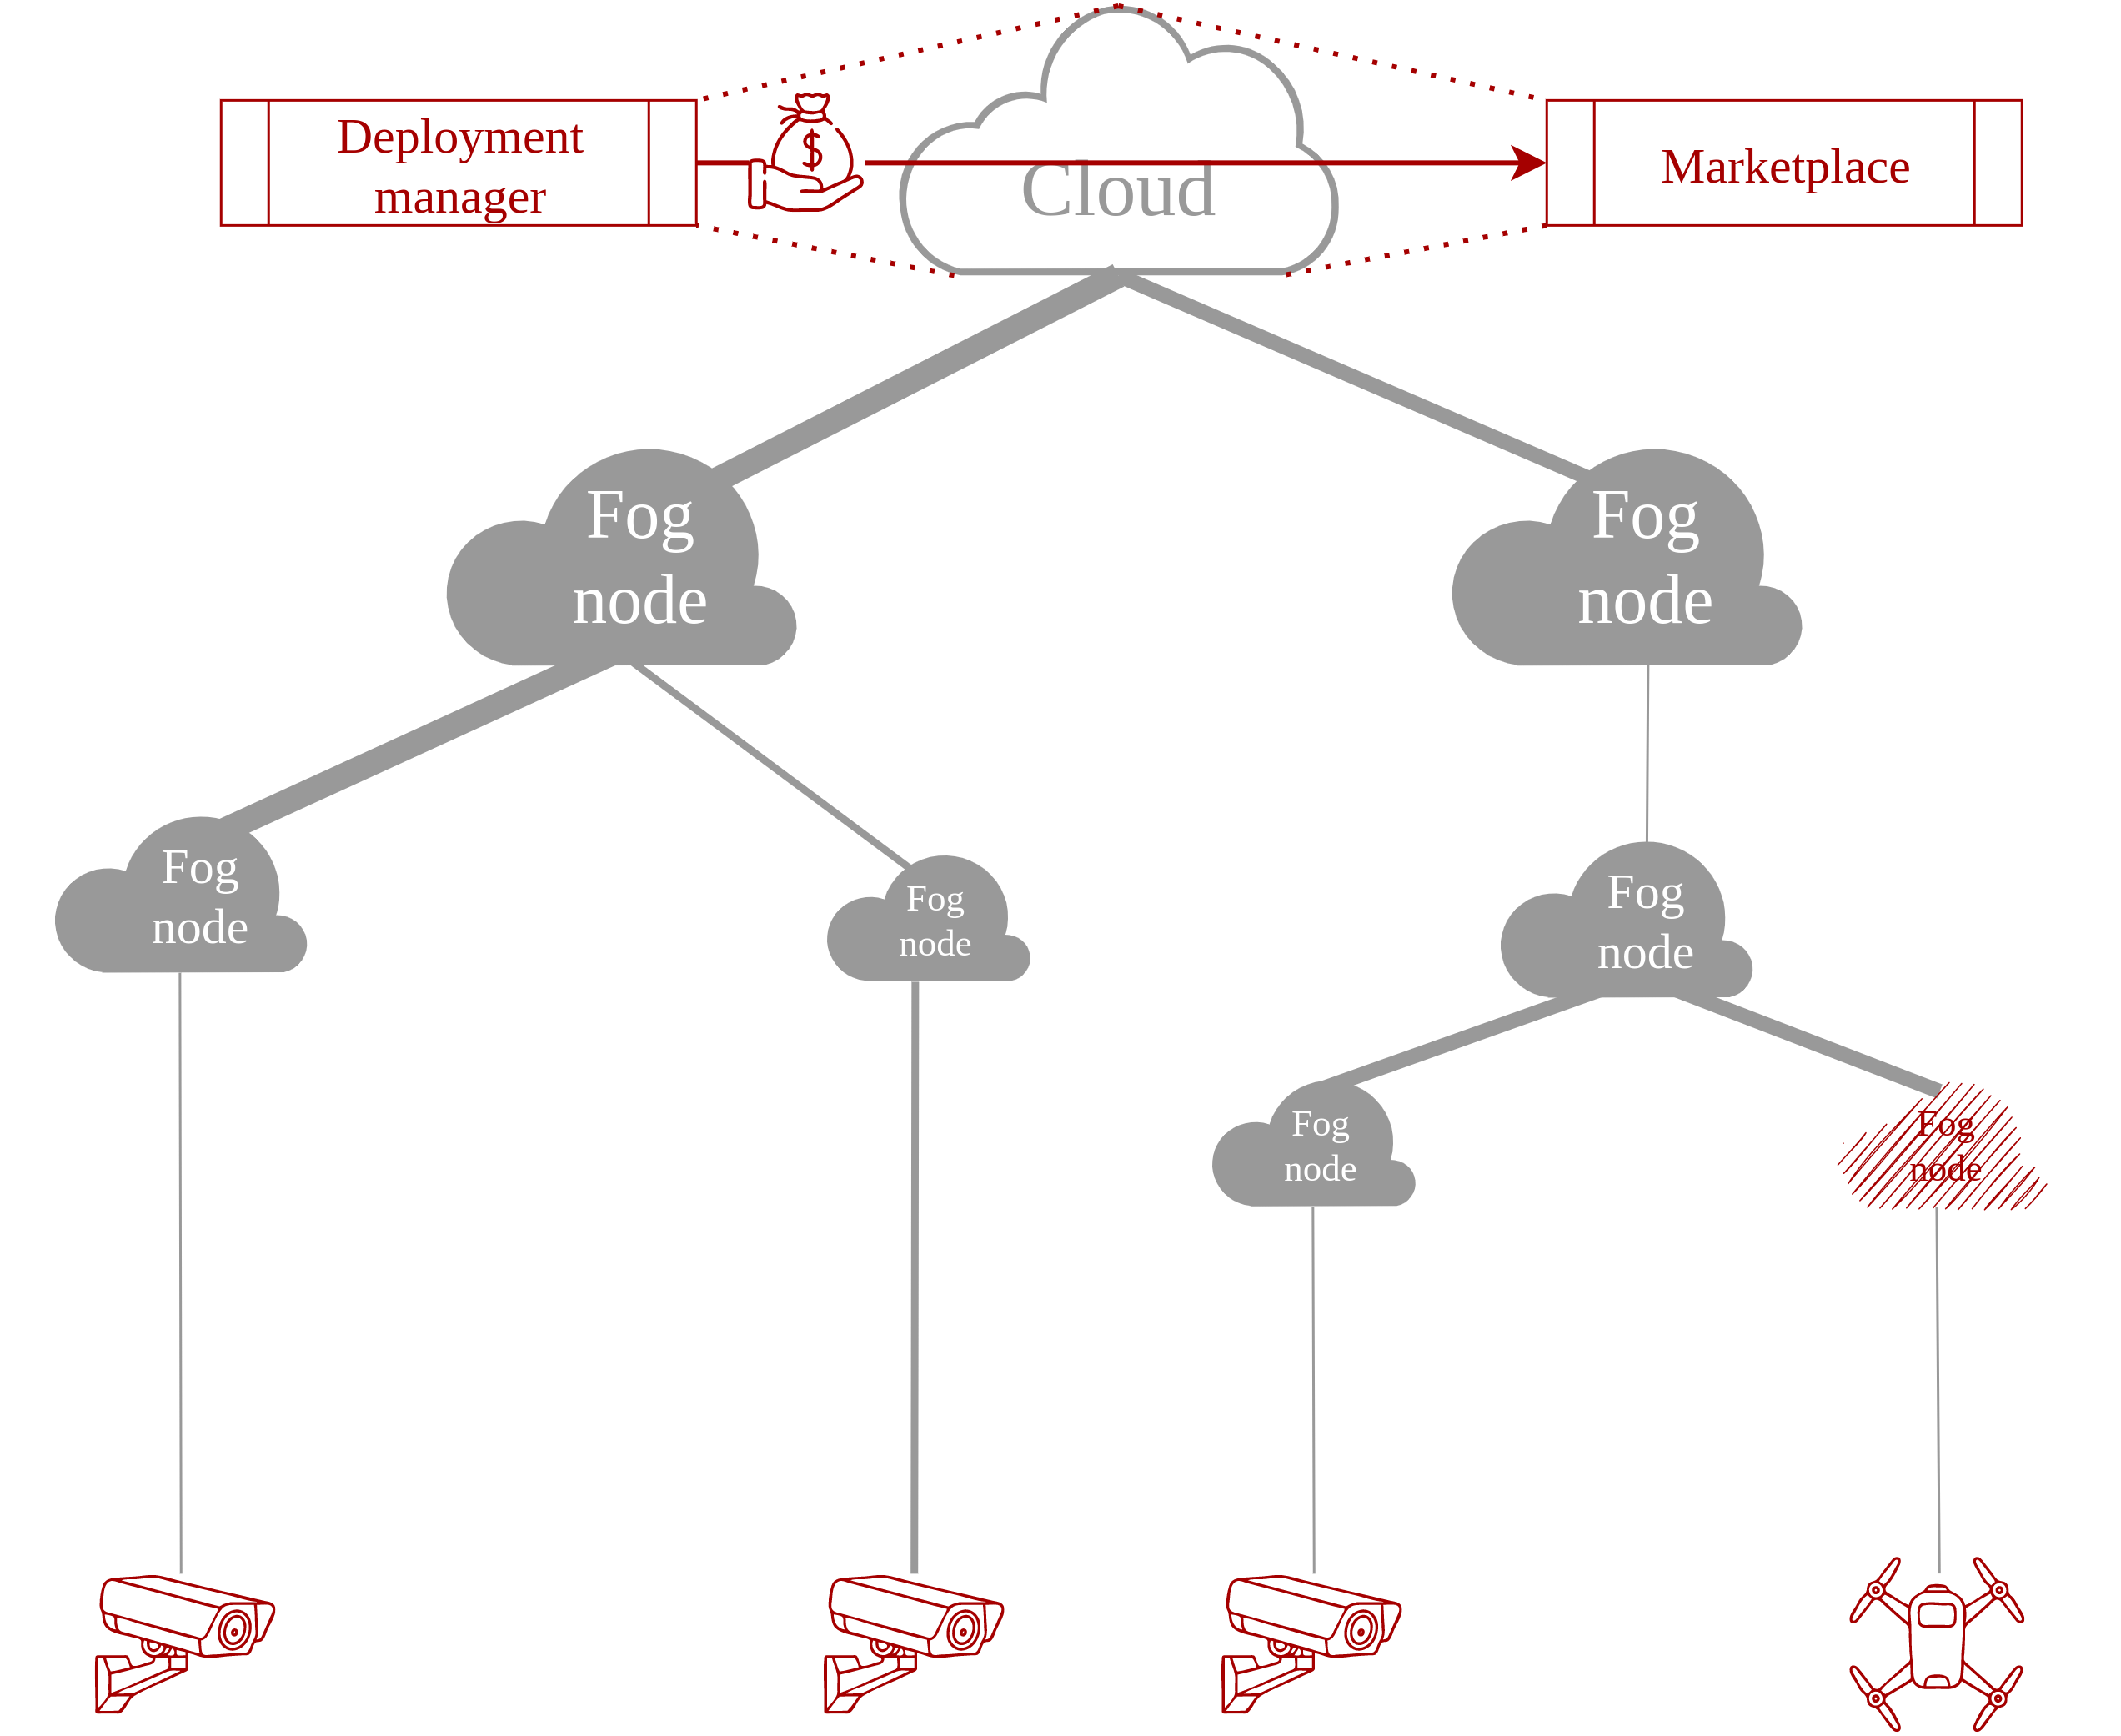
\includegraphics[width=0.65\textwidth]{./assets/OurPlacementOriginal-Page-4.png}
	\caption[Step 3—Payment and provisioning]{step 3—Payment and provisioning\\
		\textit{Once all bids have been received by the Marketplace, auctions are held a winning Fog node is given back to the Deployment Manager. The function is then instantiated as specified in the \gls{SLA}.}}
	\label{fig:our_placement3}
\end{figure}

Our placement algorithm work in four main steps\footnote{Thanks to “AmethystDesign”, “Amethyst Prime”, “SBTS2018”, “bsd” and “freepik” for their images downloaded from “flaticon.com”}:

\begin{description}
	\item[Step 0]{( \cref{fig:our_placement0}) simply answers to the question: “How do the application is made aware the necessary \gls{IoT} devices have joined to run properly?”
		The response is through a simple “ping” informing the Deployment Manager that part of its hardware is connected and it may need to take a decision to integrate it in the deployed application.
	}
	\item[Step 1]{( \cref{fig:our_placement1}) is about the creation of and \gls{SLA}. When the Deployment Manager wants to provision a new function on the Fog network, it will be their responsibility to split their applications and constitute functions that will be run on the Fog. Those functions are then described by a \gls{SLA} wrapping multiple requirements such as CPU, RAM, latency.
		
		This contract represents guarantees to the execution of the function. A key point is that we consider everything has a price in the Fog, as such, any need will be able to be provided. However the cost may be infinitely high…
		
		Once the \gls{SLA} is ready, it is sent to the Marketplace which starts the auctioning process. The first action taken is to dispatch the contract to an arbitrary Fog node in the network. Every node will then relay the \gls{SLA} until one requirement is broken.
	}
	\item[Step 2]{ (\cref{fig:our_placement2}) is the bidding process. Every fog node looks at the \gls{SLA} and bids. Thanks to an appropriate auctioning mechanism, it will represent the actual value—the truthful value—of the function through the eyes of the Fog node. We chose to go with second-price auctions, so as to have those properties when bidding on a single function. However, it is not maintained regarding multiple auctions for the same goods, like in our case. Thus in future works, we will need to consider another auctioning process. Once this process has been done, the bid is returned to the Marketplace.}
	\item[Step 3]{ (\cref{fig:our_placement3})is the final step. Here, the Marketplace received all the bids of all the suitable Fog node to execute the function. The auction takes place and the winner is given to the Deployment Manager for further action. Two options are available: not to purchase and find another strategy to achieve its goal. Or to pay the Marketplace that in turn will remunerate the Fog node that will provision the function and so, make the application work. Of course, payment will not travel to the Fog node but in parallel in order to save on precious bandwidth.}
\end{description}

I coded this strategy in a framework.

\subsubsection{Limitations of existing frameworks}

We chose to start our especial framework from scratch. In short, no other solution could have allowed us to efficiently compare multiple placement approaches as well as by introducing our own.

Our criteria were the followings:
\begin{itemize}
	\item not abandoned;
	\item extensively and painlessly modifiable (network topology, distribution process for the functions);
	\item ready to be deployed on a real test bed;
	\item can exploit Grid'5000;
	\item easily measurable;
	\item uses standard technologies so that we can benefit from already industrialized application samples and from the research literature about \gls{FaaS} optimizations methods. Thus using already updated components instead of relying on custom but simplistic implementations.
\end{itemize}

One key aspect we kept in mind was the time and efforts necessary to understand and repurpose a framework to fit our imperatives versus the time we would need to develop our own solution.

In the community, two frameworks caught our eyes.
\begin{description}
	\item[\cite{deng_fogbus2_2021}]{is a research project. However the authors chose to employ their unique implementation of the orchestration system instead of going with Kubernetes, directly resting on Docker. Furthermore, they do not advertise their framework as being suited for extensive modification that would be crucial in our case: auctions and the creation of the Marketplace are the first requirement. Thus, this framework is not sufficient for our needs.
	}
	\item[\cite{smartfog_fogflow_2022}]{ is a mature framework coming from the research world. It is the result of a two papers \cite{cheng_fogflow_2018, cheng_fog_2019} that make it what it is today: a wonderful open framework for early adopters of the Fog technology. Particularly since the project is part of the Fiware \cite{fiware_foundation_fiware_2021} backed by a number of great companies. However, for our needs, the framework is not appropriate. It is too complicated to understand fast, making modifications hard to deal with. Especially since we would have to implement the auctioning mechanisms on top of it, and enable messaging upon its existing stack. Even the underlying orchestrator is not standard. For these reasons, the framework is not interesting for us.}
\end{description}

Both of the choices look as if they are actively maintained, with an emphasize over \cite{smartfog_fogflow_2022} since the commits usually dates back days instead of months as in \cite{deng_fogbus2_2021}.
However, neither option is  sufficient for us and we proceeded with developing our own solutions, fit to our needs. An additional benefit of this is the coupling of the framework with Grid'5000 as our testing and experimental ground.

\subsubsection{A framework to rule them all}

I implemented this framework in Rust. The use of this innovative language present several benefits, in no order:
\begin{itemize}
	\item multiple targeted architectures due to the exploitation of a modern toolchain. It favors simple compilation steps for x86 (when testing on Grid'5000) and ARM (when testing on Raspberry Pi clusters, in the future), theoretically by only having to compile on an ARM platform to support that platform;
	\item Rust enables developers to be confident in their code, e.g., where Python allows typographic errors in its code, Rust forbids them by design;
	\item helpfulness of the compiler, e.g., it can detect race condition on variable access in multithreading environment;
	\item default high standard regarding code quality thanks to the Rust toolkit, making it perfect for community sharing and contributions. e.g., by default errors are handled and no exceptions rose, making the software far more reliable than the result of dynamic languages;
	\item low-level code strengths with the expressivity and simplicity of high-level code, making it ideal if the framework needs to accomplish high efficiency unforeseen tasks—such as routing;
	\item extendability through the utilization of WebAssembly, enabling diverse module integration to modify the behavior of the platform,  e.g., this would be especially useful for the decision-taking process on Fog nodes to give a bid. It would allow other languages than Rust on a small parcel of the software. Thus making the tester comfortable to experiment with various strategies in “production” and keep the clean practice of Rust processing the resulting data.
\end{itemize}

Additionally, relying on industrial components such as Kubernetes, or in a lesser extent, OpenFaaS allow us to separate concerns in the framework to only concentrate on our contributions. As a matter of facts, it would event benefit us since we could implement researched improvements on the underlying. And doing so without actually touching our framework behaviors, especially for changes like function chaining and low-level fault tolerance (local crashes on the node itself).

\todo{Maybe add things to that section}

\subsubsection{Benefits and limitations}

The development of our own framework comes with benefits and a price.

The utilization of Rust, a strongly typed language, favors the generation of standard OPEN API v3 documentation for the routes created for the \gls{REST} \gls{API}. Especially because it is so easy to go only from its typing system to a documentation presenting both the input and outputs object models to expect on the routes. This means the project can be shared as most of the endpoints are documented in their intentions and actions. Additionally, since the framework is implemented respecting the clean architecture, it eases the modification of the underlying technology, if necessary. For example, one would be able to extend the framework to use another orchestrator instead of Kubernetes—granted this would nevertheless take a great amount of time, but still, the whole application would not need to be changed. In fact, only the part that employs the communication with the orchestrator itself. This means the design enables the adjustment of the behavior of the framework regarding placement of functions, auctions, etc. A required feature when it comes to compare against state-of-the-art research placement algorithms.

The current implementation is not complete yet compared to the initial ideas. Time is a constraint. The main limitation—artificial—is the tree topology we use as a simplification. In the future, we will extend the approach to a tangible graph topology to reflect the possibilities of the real world.

Another clarification is the absence of any security and monetary mechanism. Indeed, we simplified this aspect, deemed not crucial for the purpose of research. For example, the step of payment is not implemented because it would essentially introduce a difficulty for no extra benefits to the task of function placement.

\subsubsection{Running the framework}

We planned from the beginning to execute this framework on Grid'5000.

Grid'5000 is a large-scale test bed for experimentations. It is a cluster of multiple data centers geographically scattered in research facilities, mainly in France. Every site offer from tens to hundreds of computing nodes ready for experiment. Each node is customizable from its kernel to the software that runs on it. Further configurations include networking and the size of the virtual instances, i.e., the resources reserved.

This way we can profit from a rigorous test environment in which to run reproducible studies thanks to a level of control not available in public Clouds. Another key point is scalability. We can expand our Fog network to any arbitrary number of nodes to experimentally validate our concepts. The addition of both benefits enables us to select the resources allowed per Fog nodes, and network conditions in between the nodes. Thus, we can perfectly model the Fog experimentally. For our utilization, we primarily focus on bandwidth and latency. Indeed, the constraints on the resources will come after having proven the framework is able to run on a network stack matching the Fog.

Employing Grid'5000 can be achieved in several ways. The first—the legacy one—is through SSH and the execution of a number of bash scripts that create and control both the environment and the flow of the experiment.
Another manner has been introduced thanks to the development of EnosLib \cite{cherrueau_enoslib_2022}. This library allows the complete use of Grid'5000 as the legacy, with one catch. One does not have to cope with the documentation of Grid'5000 and learn its specific technical subtilities and tricks to make matters work. Everything is included in this Python library. Of course, documentation is still necessary to appreciate the various functionalities, but when lacking, one does have another way to solve their trouble. Instead of relying on bothering people through a mailing list, one can access the source code and understand the implementation. That way it usually takes less time than to explain the problem to a third party—particularly thanks to the code being commented.

Thanks to this library, a command line wrapper can be created easily. The resulting script is more straightforward than utilizing a bunch of bash scripts, especially since it is run on the developer's hardware. Every SSH trick, copy, redirection and even standard installations are handled. For example, using Docker is as simple as instantiating a Python context stating to run Docker, see the code below in \cref{listing:dockerenos}.

\begin{lstlisting}[language=Python, caption=EnosLib context example with Docker, label=listing:dockerenos]
	with en.Docker(agent=roles['builder']):    # Install Docker
	try:
	res = en.run_command(                  # Run a command
	'docker build -t fog_node:latest .', # A bash command using Docker
	roles=roles['builder'])              # Specify on what machines to act on
	except EnosFailedHostsError as err:
	pass
\end{lstlisting}

However, executing bash commands is still an available option, but now, one does not need to care about the specificities of the nodes such as their IP, regardless of whether they are running a virtual machine, etc. Commands are automatically dispatched to the appropriate machines given their role—a tag.

So this fastens development time by a lot. Another compelling feature that I will be employing in the extremely near future is the data gathering. This library has been thought to be managing experiments, and as such, simplifies data collection. This engaging aspect is the use of Prometheus endpoints.

Prometheus \cite{prometheus_authors_prometheus_nodate} is a monitoring solution providing the necessities to that reach that goal: time series logging, advanced queries, data visualization, storage, alerting, numerous integrations. This open-source project hosted by the Cloud-native Foundation collects and store metrics with their timestamps in a database. In our particular case of deploying software on multiple computing nodes, it makes it easy to centralize, accumulate all the measurements for later exploitation.

With the use of appropriate crates (libraries) in Rust \cite{sully_rocket_prometheus_2022}, I would be capable to produce compatible endpoints on my framework. Those will be linked to EnosLib through Prometheus and record interesting metrics: latency between Fog nodes, load on the Fog node, number of instantiated functions, etc.

\subsubsection{Our evaluation plan}

We plan to evaluate the framework to release a paper by the end of my internship \improvement{State the end of the internship in the introduction}. To do so, we divided our strategy into two levels, in order to at least be able to publish a straightforward statement to tell the community that this framework is in the works.

\begin{description}
	\item[Level 1]{is the comparison of our auctioning strategy with naive Fog fillings. Such fillings are loading the network from the top, or respectively, from the bottom. This way benefits of our method and proof of the extensibility of the framework can be gauged.}
	\item[Level 2]{is the comparison against state-of-the-art placement algorithms. Our goal is to identify and measure key differences of our approach with \cite{tasiopoulos_fogspot_2019, bermbach_auctionwhisk_2021}.}
\end{description}

Our criteria would be
\begin{itemize}
	\item deployment time;
	\item \gls{QoS};
	\item economic efficiency;
	\item fairness of the auctions;
	\item scaling potential.
\end{itemize}

Economic efficiency aims to examine whether the Fog node earns enough “money” to be lucrative for its owner. Profitability would be an incentive for the node to stay in the network. One experience could look at “what happens when unremunerative nodes leave the grid because they went bankrupt?”

\subsection{Other work accomplished}

Developing the framework was not the first work to be started. Initially, I had to be at ease with the literature of the fields this project interacts with. I wanted to go furhter about what was previously accomplished in the bibliographic report in terms of:
\begin{enumerate}
	\item placement algorithm;\label{enumerate:placement}
	\item already tested/simulated auctions;\label{enumerate:alreadytested}
	\item existing frameworks and their limitations;\label{enumerate:frameworklimitations}
	\item finding Fog applications to run on a framework.\label{enumerate:fogapplications}
\end{enumerate}

This meant a number of hours dedicated to discover an answer to those questions and go further than the bibliographic report. \cref{enumerate:placement,enumerate:alreadytested,enumerate:frameworklimitations} lead to the initiative of a new framework fitting our particular needs and profiting from advantages such as Grid'5000—that kind of test bed is not usual in the domain literature.

\cref{enumerate:fogapplications} led to uncover BeFaaS \cite{grambow_befaas_2021}. This paper uses an openly available Fog application to benchmark \gls{FaaS} platforms. It proposes a traffic light application aware of the kind of vehicle (cars, ambulances, etc.) circulating through it and the weather conditions and takes traffic management decisions from those data. Though it is still an artificial application—the image recognition part is basically pixel remapping on a fake image in order to “simulate” the computational cost of recognition. It is the closest I observed to a Fog application.

Of course a number of \gls{FaaS} applications are available \cite{eskandani_wonderless_2021}. However one would have to go through all the different technologies to find code compatible with a platform. This entanglement is particularly visible with open private Cloud products—such as AWS' \cite{tarneberg_experiences_2016,eismann_state_2021}. Meaning reusing the code is not possible without both redoing it and logically replacing its components, e.g., migrate storage solutions and triggers. Ultimately, the main issue with this approach is that those applications are not custom tailored for the Fog. What we want is to first investigate Fog applications made for this platform and only then, test normal applications to complete the study of the state of Fog integration with current Cloud offerings.

Finally, we went with BeFaaS \cite{grambow_befaas_2021} and actually rewrote their simple application with Rust in order to:
\begin{itemize}
	\item get rid of their library incorporation that they created for their experiments—thus not using all the features (asynchronous calls) of our picked platform: OpenFaaS;
	\item get rid of Terraform, as it would have been an annoying additional layer to manage for no benefits;
	\item get rid of JavaScript, as this would be a doubtful choice for a “high-performance” language employed for applications running under constraints, and likely paying for their resource consumptions.
\end{itemize}
In the end, the application was rewritten in Rust and that uplifted the whole project as I also planned to utilize this language for the framework itself. Hence it was an excellent training and way to find the appropriate crates—aka modules—that I would later utilize in the framework. A good example is the crate I retained for the \gls{REST} \gls{API}, with which I was hesitant to go at first, but after testing another option I realized the benefits of Rocket \cite{benitez_rocket_2022} and so I went with it for the framework.

\subsubsection{Plans of evolution and future research work}

“Flexible resource allocation for \gls{FaaS} applications in the Fog” is the title of my thesis.
I earned the funding through the XXXXX. \todo{Put the name of the contest} thanks to the good advice of Nikos, under whose supervision I will research this topic.

The main point in altering the first words in the sentence is to reflect the change of scope. Instead of just focusing on the function placement, which is a one-time event that occurs at the provision of the function; we now look at the life of the application in the Fog. Of course the application will be divided in functions, but then those will require to stay linked with each other, to move in the Fog to maintain meeting their specifications. And by doing so, the auctioning process will need to integrate those changes, as to keep fairness during all operations for all users, etc.

\begin{figure}[H]
	\centering
	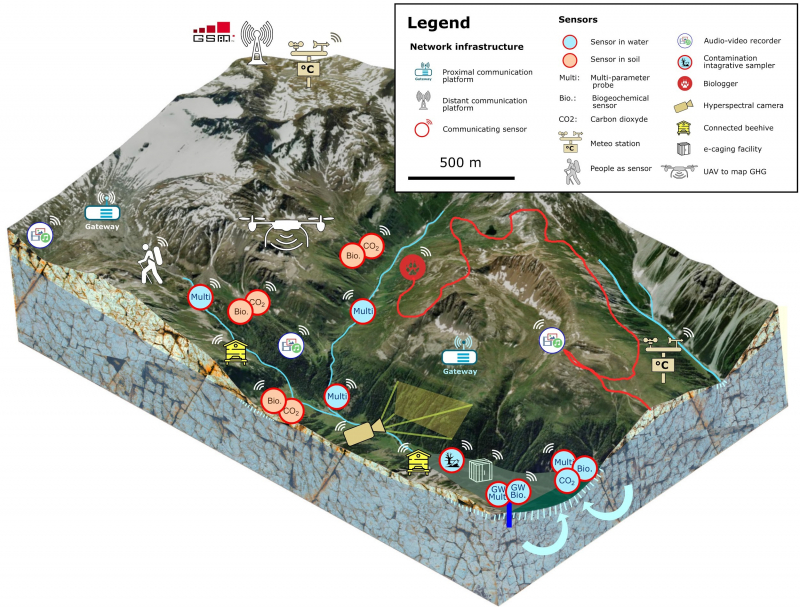
\includegraphics[width=1\textwidth]{./assets/terraforma.jpg}
	\caption[What a Terra Forma observatory could look like]{What a Terra Forma observatory could look like.\\
		\textit{A site combining both mobile and static connected sensors and platforms. © Virginie Girard, Laurent Longuevergne, Arnaud Elger}}
	\label{fig:terraforma}
\end{figure}

We also want to participate in the Terra Forma \cite{longuevergne_terra_2022} CNRS-backed mission to both help and experiment on an actual Fog test bed. Indeed the project will monitor part of the French territory under a dense net of multiple \gls{IoT} sensors. We hope to demonstrate the power of the Fog reducing bandwidth consumption and enabling real-time decision taking (drone control, etc.). In such a project, we will be able to contribute our framework running in the real world, our placement mechanism as well as an economically viable solution and, lastly, true Fog applications at scale—a still scarce sight in the literature.

\section{Conclusion}
% Financial cooperation as key

\todo{add internship to conclusion}

Serverless, and especially \gls{FaaS}, enables the transfer of resource provisioning responsibilities to the platform provider. Thus, this model enables orchestration optimizations in resource-usage, data transfers, virtualization, etc. The model could be viable in the Fog because functions are light enough to be provisioned on multiple constrained devices, and when placed strategically, scale dynamically over the network by design.

This report presents an overview of contributions made to the state of the art when it comes to function placement in highly distributed systems—either Fog or \gls{MEC}. These contributions address open questions such as \cite{kjorveziroski_iot_2021,xie_when_2021}:
\begin{enumerate}[(a)]
	\item scheduling;
	\item deployment;
	\item performance;
	\item cold-start;
	\item vendor lock-in;
	\item security \& isolation;
	\item improvement to function chaining / combination;
	\item support for hardware acceleration (\gls{GPU}, \gls{APU}, \gls{AI}, etc.);
	\item resource awareness and service discovery;
	\item incentive mechanism;
	\item exceptions and failure recovery.
\end{enumerate}
After synthesizing the knowledge in \cref{tab:placement}, new questions are raised about
\begin{enumerate}[(i)]
	\item the role of \glspl{SLA} and the guarantees they could provide for the Fog and its users;
	\item an auction-based model that would translate the complexity of users' needs in meaningful bids, helping to place truthfully and fairly functions on nodes;
	\item the integration of \gls{FaaS} and their inherent constraints in the Fog;
	\item the place of security and privacy.
\end{enumerate}